%!TEX program = xelatex
\documentclass[dvipsnames, svgnames,a4paper,11pt]{article}
% ----------------------------------------------------
%   中山大学物理与天文学院本科实验报告模板
%   作者:Huanyu Shi,2019级
%   知乎:https://www.zhihu.com/people/za-ran-zhu-fu-liu-xing
%   Github:https://github.com/huanyushi/SYSU-SPA-Labreport-Template
%   Last update : 2023.4.10
% ----------------------------------------------------

% ----------------------------------------------------- 
%	加边框的命令
%	参考:https://tex.stackexchange.com/questions/531559/how-to-add-the-page-border-for-first-two-pages-in-latex
\usepackage{tikz}
\usetikzlibrary{calc}
\usepackage{eso-pic}
\AddToShipoutPictureBG{%
\begin{tikzpicture}[overlay,remember picture]
\draw[line width=0.6pt] % 边框粗细
    ($ (current page.north west) + (0.6cm,-0.6cm) $)
    rectangle
    ($ (current page.south east) + (-0.6cm,0.6cm) $); % 边框位置
\end{tikzpicture}}


\usepackage{xcolor}
\definecolor{c1}{HTML}{2752C9} % 目录颜色
\definecolor{c2}{RGB}{190,20,83} % 引用颜色

\usepackage{ctex}
\usepackage[top=28mm,bottom=28mm,left=15mm,right=15mm]{geometry}
\usepackage{hyperref} 
\hypersetup{
	colorlinks,
	linktoc = section, % 超链接位置,选项有section, page, all
	linkcolor = c1, % linkcolor 目录颜色
	citecolor = c1  % citecolor 引用颜色
}
\usepackage{amsmath,enumerate,multirow,float}
\usepackage{tabularx}
\usepackage{tabu}
\usepackage{subfig}
\usepackage{fancyhdr}
\usepackage{graphicx}
\usepackage{wrapfig}  
\usepackage{physics}
\usepackage{appendix}
\usepackage{amsfonts}

%
\usepackage{tcolorbox}
\tcbuselibrary{skins,breakable}
\newtcolorbox{tbox}[2][]{
    colframe=black!70!,
    breakable,
    enhanced,
	boxrule =0.5pt,
    title = {#2},
    fonttitle = \large\kaishu\bfseries,
	drop fuzzy shadow,
    #1
}
\newtcolorbox[auto counter,number within=section]{question}[1][]{
  top=2pt,bottom=2pt,arc=1mm,
  boxrule=0.5pt,
%   frame hidden,
  breakable,
  enhanced, %跨页后不会显示下边框
  coltitle=c1!80!gray,
  colframe=c1,
  colback=c1!3!white,
  drop fuzzy shadow,
  title={思考题~\thetcbcounter:\quad},
  fonttitle=\bfseries,
  attach title to upper,
  #1
}

% ---------------------------------------------------------------------
%	利用cleveref改变引用格式,\cref是引用命令
\usepackage{cleveref}
\crefformat{figure}{#2{\textcolor{c2}{图 #1}}#3} % 图片的引用格式
\crefformat{equation}{#2{(\textcolor{c2}{#1})}#3} % 公式的引用格式
\crefformat{table}{#2{\textcolor{c2}{表 #1}}#3} % 表格的引用格式


% ---------------------------------------------------------------------
%	页眉页脚设置
\fancypagestyle{plain}{\pagestyle{fancy}}
\pagestyle{fancy}
\lhead{\kaishu 中山大学物理与天文学院近代物理实验\uppercase\expandafter{\romannumeral1}} % 左边页眉,学院 + 课程
\rhead{\kaishu D8 \quad 氦氖激光综合实验} % 右边页眉,实验报告标题
\cfoot{\thepage} % 页脚,中间添加页码


% ---------------------------------------------------------------------
%	对目录、章节标题的设置
\renewcommand{\contentsname}{\centerline{\huge 目录}}
\usepackage{titlesec}
\usepackage{titletoc}
% \titleformat{章节}[形状]{格式}{标题序号}{序号与标题间距}{标题前命令}[标题后命令]
\titleformat{\section}{\centering\LARGE\songti}{}{1em}{}

% ---------------------------------------------------------------------
%   listing代码环境设置
\usepackage{listings}
\lstloadlanguages{python}
\lstdefinestyle{pythonstyle}{
backgroundcolor=\color{gray!5},
language=python,
frameround=tftt,
frame=shadowbox, 
keepspaces=true,
breaklines,
columns=spaceflexible,                   
basicstyle=\ttfamily\small, % 基本文本设置,字体为teletype,大小为scriptsize
keywordstyle=[1]\color{c1}\bfseries, 
keywordstyle=[2]\color{Red!70!black},   
stringstyle=\color{Purple},       
showstringspaces=false,
commentstyle=\ttfamily\scriptsize\color{green!40!black},%注释文本设置,字体为sf,大小为smaller
tabsize=2,
morekeywords={as},
morekeywords=[2]{np, plt, sp},
numbers=left, % 代码行数
numberstyle=\it\tiny\color{gray}, % 代码行数的数字字体设置
stepnumber=1,
rulesepcolor=\color{gray!30!white}
}




% ---------------------------------------------------------------------
%	其他设置
\def\degree{${}^{\circ}$} % 角度
\graphicspath{{./images/}} % 插入图片的相对路径
\allowdisplaybreaks[4]  %允许公式跨页 % 导入模板的相关设置
\usepackage{lipsum}
\usepackage{enumitem}
\usepackage{tabularray}  % 绘制表格时可以更加方便添加框线
\usepackage{diagbox}	% 方便给表格添加对角线
\setlist[enumerate]{label=\textup{(\arabic*)}}



%---------------------------------------------------------------------
%	正文
%---------------------------------------------------------------------

\begin{document}


\begin{table}
	\renewcommand\arraystretch{1.7}
	\begin{tabularx}{\textwidth}{
		|X|X|X|X
		|X|X|X|X|}
	\hline
	\multicolumn{2}{|c|}{预习报告}&\multicolumn{2}{|c|}{实验记录}&\multicolumn{2}{|c|}{分析讨论}&\multicolumn{2}{|c|}{总成绩}\\
	\hline
	\LARGE25 & & \LARGE30 & & \LARGE25 & & \LARGE80 & \\
	\hline
	\end{tabularx}
\end{table}


\begin{table}
	\renewcommand\arraystretch{1.7}
	\begin{tabularx}{\textwidth}{|X|X|X|X|}
	\hline
	专业:& 物理学 &年级:& 2022级\\
	\hline
	姓名:& 戴鹏辉  & 学号: & 2344016 \\
	\hline
	日期:& 2024/9/20 & 教师签名:& \\
	\hline
	\end{tabularx}
\end{table}

\begin{center}
	\LARGE D1 \quad 锁相放大器与弱信号测量
\end{center}

\textbf{【实验报告注意事项】}
\begin{enumerate}
	\item 实验报告由三部分组成:
	\begin{enumerate}
		\item 预习报告:(提前一周)认真研读\underline{\textbf{实验讲义}},弄清实验原理;实验所需的仪器设备、用具及其使用(强烈建议到实验室预习),完成课前预习思考题;了解实验需要测量的物理量,并根据要求提前准备实验记录表格(第一循环实验已由教师提供模板,可以打印)。预习成绩低于10分(共20分)者不能做实验。
	    \item 实验记录:认真、客观记录实验条件、实验过程中的现象以及数据。实验记录请用珠笔或者钢笔书写并签名(\textcolor{red}{\textbf{用铅笔记录的被认为无效}})。\textcolor{red}{\textbf{保持原始记录,包括写错删除部分,如因误记需要修改记录,必须按规范修改。}}(不得输入电脑打印,但可扫描手记后打印扫描件);离开前请实验教师检查记录并签名。
	    \item 分析讨论:处理实验原始数据(学习仪器使用类型的实验除外),对数据的可靠性和合理性进行分析;按规范呈现数据和结果(图、表),包括数据、图表按顺序编号及其引用;分析物理现象(含回答实验思考题,写出问题思考过程,必要时按规范引用数据);最后得出结论。
	\end{enumerate}
	\textbf{实验报告就是将预习报告、实验记录、和数据处理与分析合起来,加上本页封面。}
	\item 每次完成实验后的一周内交\textbf{实验报告}(特殊情况不能超过两周)。
	% \item 实验报告注意事项
	% 	\begin{enumerate}[label=\roman*.]
	% 		\item 
	% 	\end{enumerate}
\end{enumerate}


\clearpage
\tableofcontents
\clearpage

\setcounter{section}{0}
\section{D1 \quad 锁相放大器与弱信号测量——【实验1】锁相放大器工作原理、基本参数与基本操作 \quad\heiti 预习报告}
	
\subsection{实验目的}
\begin{enumerate}
	\item 了解锁相放大器工作原理和特点, 理解信号、 噪声、 信噪比等概念。
	\item 掌握锁相放大器基本参数含义及锁相放大器的基本操作, 学会合理选择或调节参数( 频率、 相位、 灵敏度、 时间常数、 陡降) ; 复习示波器的使用;
	\item 掌握用锁相放大器检测弱信号方法, 通过与示波器比较其检测能力了解其技术优势。
	
\end{enumerate}

\subsection{仪器用具}
\begin{table}[htbp]
	\centering
	\renewcommand\arraystretch{1.6}
	% \setlength{\tabcolsep}{10mm}
	\begin{tabular}{p{0.05\textwidth}|p{0.20\textwidth}|p{0.05\textwidth}|p{0.5\textwidth}}
	\hline
	编号& 仪器用具名称 & 数量 &  主要参数(型号,测量范围,测量精度等) \\
	\hline
	1	&	锁相放大器 	&1 	& OE1022( 系列)\\

	2	&	配套教学实验箱 	&1 	& 		 \\
	
	3	&	示波器 & 1 &	RIGOL DS2202A 	\\
	
	4	&	信号发生器	&1 & RIGOL DG4162	\\
	
	5	&	BNC-BNC 信号线	&	若干 & \\
	\hline
\end{tabular}
\end{table}

\subsection{原理概述}


	




\subsection{实验前思考题}

% 思考题1
\begin{question}
	市频 50Hz 干扰通常通过电源耦合,影响仪器的测量结果;对于 997Hz 的待测信号,50Hz 干扰是噪声吗?对锁相放大器的测量会有影响吗?
\end{question}

市频 50Hz 干扰主要通过电源线或其他电磁耦合路径引入到测量系统中,表现为一种低频的正弦信号。由于 50Hz 是非常常见的环境噪声源,许多实验仪器在测量过程中都会受到此频率的干扰。在实验中,50Hz 干扰可以被视为一种不相关的噪声。它与 997Hz 的待测信号频率明显不同,因此可以认为是一种外部噪声源。锁相放大器的一个主要功能就是从噪声背景中提取出目标信号,所以关键问题是 50Hz 的干扰是否会影响锁相放大器的测量。

待测信号的频率为 997Hz,而 50Hz 干扰频率与待测信号相差很大。理论上,锁相放大器会根据设置的参考频率(997Hz)来进行锁定,因此 50Hz 干扰会被滤除,并不会直接影响测量结果。

虽然锁相放大器能够在频率上选择性滤除不相关的噪声,但 50Hz 干扰仍有可能产生一些间接的影响。50Hz 干扰可能会产生 100Hz、150Hz 等谐波成分,这些频率成分接近或落在待测信号附近时,可能会引起较小的干扰,尤其是当谐波频率接近参考频率时,滤波器的效果会降低。50Hz 干扰可能引入低频的基线漂移,增加测量的不稳定性。如果干扰信号的幅度较大,可能会使得信号源的供电或参考信号不稳定,从而影响实验的重复性。

尽管锁相放大器能部分解决这个问题,但还是有一些额外的措施可以进一步降低50Hz干扰的影响。确保实验设备和电缆有良好的屏蔽,并做好接地工作,以减少电磁耦合带来的干扰。在锁相放大器的输入端加装陷波滤波器(50Hz陷波器),专门抑制 50Hz 的干扰信号。尽量远离大型电气设备或电源线,以减少市电干扰的耦合。
	


% 思考题2
\begin{question}
	如何用锁相放大器检测到待测的直流信号或慢变信号?(图 D1-9 中的$v(t)$为直流或慢变信号)
\end{question}

锁相放大器的主要功能是从噪声背景中提取特定频率的信号。它通过将输入信号与参考信号(通常是一个正弦波)相乘,生成调制信号。然后,低通滤波器滤除与参考频率不同的成分,只保留同频率且相位一致的部分。这使锁相放大器在高噪声环境中非常有效,尤其是对于交流(AC)信号的提取。然而,锁相放大器的这种原理主要是为交流信号设计的,因此对于直流(DC)信号或缓慢变化的信号(低频信号),需要采取一些额外措施来适应其检测。

锁相放大器通常依赖于参考信号来选择性放大输入信号中的某个频率。如果待测信号是直流信号或频率非常低,它不会与常规交流参考信号匹配,难以直接应用常规的锁相放大技术。在直流信号情况下,如果直接通过锁相放大器来测量,由于没有与直流信号相对应的调制参考信号,锁相放大器会无法区分直流信号和直流偏置的噪声。因此,直接检测直流信号的有效性有限。

要检测直流或慢变信号,常用的方法是对信号进行调制,将其变为交流信号,然后使用锁相放大器检测调制后的信号。

斩波调制(Chopping modulation)是一种常见的方法,尤其在光学检测中。例如,假设你要测量某个光电探测器的输出信号,该输出信号可能是缓慢变化的或接近直流。通过使用一个机械或电子斩波器,信号可以被调制为一个周期性的方波或正弦波。斩波器的频率通常设置在数百赫兹到千赫兹的范围内,这个频率同时作为锁相放大器的参考频率。经过调制后的信号从直流或慢变信号变成了一个与参考信号相匹配的交流信号,锁相放大器可以通过对调制频率进行锁定,检测出该调制后的信号。调制的优点是将低频或直流信号从低频噪声(如 1/f 噪声)中分离出来,显著提高信噪比。

另一种方法是引入一个外部调制器,使信号周期性地变化。例如,给待测的直流信号添加一个已知频率的小振幅交流调制。这个交流调制信号将与直流信号一起被输入到锁相放大器中,通过锁相放大器锁定该已知频率,可以提取出信号的幅度和相位信息。该方法广泛应用于许多领域,比如在激光光学系统中,通过给激光源施加调制,可以从背景噪声中提取目标信号。

对于慢变信号,虽然其频率较低,但仍是一个交流信号,可以通过适当的锁相放大器设置进行检测。锁相放大器的参考频率应与待测慢变信号的频率相匹配。由于信号变化缓慢,因此可以将参考频率设定得较低,甚至可以是毫赫兹级别。这样可以确保信号与参考信号的相位匹配,锁相放大器仍能有效检测到信号。对于慢变信号,锁相放大器的低通滤波器时间常数应适当增加。较长的时间常数可以减少高频噪声干扰,稳定慢变信号的检测。

检测直流或慢变信号时,由于信号频率低,系统中低频噪声的影响会显得更加明显。例如,1/f 噪声和温度漂移可能成为主要干扰源。因此,良好的屏蔽、接地和温控是保证实验精度的关键。在调制方法中,确保调制器和锁相放大器的同步性至关重要。如果两者不同步,信号提取可能会失败或产生较大误差。



% 思考题3
\begin{question}
	如用斩波器调制直流信号(如光强),被斩制后的信号(图 D1-9 中的$u_m(t)$信号)仍然包含有直流分量(即平均值不为零),但该直流分量随交流信号输入锁相放大器后不会被锁相放大器检测,请从数学推导上说明。
\end{question}

首先,直流信号(例如光强)经过斩波器调制,变成了一个周期性的交流信号。斩波器通常会将信号切换为一个方波或其他周期性波形。

设原始直流信号为:

\[
S_{\text{DC}}(t) = A
\]

其中,\( A \) 是直流信号的幅度。

斩波器的调制函数 \( M(t) \) 可以表示为一个方波,其值在 0 和 1 之间变化,频率为 \( f_{\text{chop}} \):

\[
M(t) = \dfrac{1}{2} + \dfrac{2}{\pi} \sum_{n=1,3,5,\dots}^{\infty} \dfrac{1}{n} \sin(2\pi n f_{\text{chop}} t)
\]

因此,经过斩波器后的信号 \( S_{\text{chop}}(t) \) 为:

\[
S_{\text{chop}}(t) = S_{\text{DC}}(t) \cdot M(t) = A \cdot M(t)
\]

将 \( M(t) \) 展开为傅里叶级数后,发现它包含一个直流分量和一系列谐波分量。

斩波信号 \( S_{\text{chop}}(t) \) 可表示为:

\[
S_{\text{chop}}(t) = A \left( \dfrac{1}{2} + \dfrac{2}{\pi} \sum_{n=1,3,5,\dots}^{\infty} \dfrac{1}{n} \sin(2\pi n f_{\text{chop}} t) \right)
\]

其中,直流分量为\( \dfrac{A}{2} \),交流分量包含频率为 \( f_{\text{chop}} \) 的基波和其奇数次谐波。

参考信号 \( R(t) \) 通常是一个与斩波器同步的正弦波:

\[
R(t) = \sin(2\pi f_{\text{ref}} t + \phi)
\]

由于斩波器的频率就是我们希望检测的信号频率,所以 \( f_{\text{ref}} = f_{\text{chop}} \)。

为了简化,设相位差 \( \phi = 0 \):

\[
R(t) = \sin(2\pi f_{\text{chop}} t)
\]

将 \( S_{\text{chop}}(t) \) 与 \( R(t) \) 相乘,得到乘法器输出信号 \( S_{\text{mix}}(t) \):

\[
S_{\text{mix}}(t) = S_{\text{chop}}(t) \cdot R(t) = A \cdot M(t) \cdot \sin(2\pi f_{\text{chop}} t)
\]

将 \( M(t) \) 展开并代入:

\[
S_{\text{mix}}(t) = A \left( \dfrac{1}{2} + \dfrac{2}{\pi} \sum_{n=1,3,5,\dots}^{\infty} \dfrac{1}{n} \sin(2\pi n f_{\text{chop}} t) \right) \sin(2\pi f_{\text{chop}} t)
\]

展开后:

\[
S_{\text{mix}}(t) = \dfrac{A}{2} \sin(2\pi f_{\text{chop}} t) + \dfrac{2A}{\pi} \sum_{n=1,3,5,\dots}^{\infty} \dfrac{1}{n} \sin(2\pi n f_{\text{chop}} t) \sin(2\pi f_{\text{chop}} t)
\]

利用三角恒等式:

\[
\sin A \sin B = \dfrac{1}{2} [\cos(A - B) - \cos(A + B)]
\]

对第二项进行展开:

\[
\sin(2\pi n f_{\text{chop}} t) \sin(2\pi f_{\text{chop}} t) = \dfrac{1}{2} \left[ \cos(2\pi (n - 1) f_{\text{chop}} t) - \cos(2\pi (n + 1) f_{\text{chop}} t) \right]
\]

因此,乘法器输出可表示为:

\[
\begin{aligned}
	S_{\text{mix}}(t) = & \dfrac{A}{2} \sin(2\pi f_{\text{chop}} t) \\
	& + \dfrac{2A}{\pi} \sum_{n=1,3,5,\dots}^{\infty} \dfrac{1}{n} \cdot \dfrac{1}{2} \left[ \cos(2\pi (n - 1) f_{\text{chop}} t) - \cos(2\pi (n + 1) f_{\text{chop}} t) \right] \\
	= & \dfrac{A}{2} \sin(2\pi f_{\text{chop}} t) + \dfrac{A}{\pi} \sum_{n=1,3,5,\dots}^{\infty} \dfrac{1}{n} \left[ \cos(2\pi (n - 1) f_{\text{chop}} t) - \cos(2\pi (n + 1) f_{\text{chop}} t) \right]
\end{aligned}
\]

低通滤波器的输入信号是 \( S_{\text{mix}}(t) \),其中包含以下频率分量:第一项,\( \dfrac{A}{2} \sin(2\pi f_{\text{chop}} t) \) —— 频率为 \( f_{\text{chop}} \) 的交流分量。第二项,由谐波生成的一系列余弦函数,频率为 \( (n \pm 1) f_{\text{chop}} \)。

为了找到低通滤波器输出的直流分量,我们需要找出在 \( S_{\text{mix}}(t) \) 中频率为零的项。

观察第二项中的 \( \cos(2\pi (n - 1) f_{\text{chop}} t) \),当 \( n = 1 \) 时:

\[
\cos(2\pi (1 - 1) f_{\text{chop}} t) = \cos(0) = 1
\]

对应的系数为:

\[
\dfrac{A}{\pi} \cdot \dfrac{1}{1} = \dfrac{A}{\pi}
\]

因此,直流分量为:

\[
S_{\text{DC,out}} = \dfrac{A}{\pi}
\]

锁相放大器的输出电压 \( V_{\text{out}} \) 与输入信号中与参考信号同频且同相的分量成正比:

\[
V_{\text{out}} \propto \langle S_{\text{chop}}(t) \cdot R(t) \rangle
\]

其中 \( \langle \cdot \rangle \) 表示经过低通滤波器后的平均值。

虽然在乘法器输出后出现了直流分量 \( \dfrac{A}{\pi} \),但这个直流分量来源于高频信号的互相作用(例如 \( n = 1 \) 的谐波与参考信号相乘得到的结果)。这些直流分量与输入信号中我们关心的那部分(与参考信号同频且同相的分量)无关。

锁相放大器的核心在于相敏检测,即它只对输入信号中与参考信号频率和相位匹配的分量敏感。

我们可以计算锁相放大器输出对直流分量的响应:

锁相放大器输出:

\[
V_{\text{out}} \propto \langle S_{\text{chop}}(t) \cdot R(t) \rangle = \langle A \cdot M(t) \cdot \sin(2\pi f_{\text{chop}} t) \rangle
\]

将 \( M(t) \) 代入:

\[
V_{\text{out}} \propto A \left\langle \left( \dfrac{1}{2} + \dfrac{2}{\pi} \sum_{n=1,3,5,\dots}^{\infty} \dfrac{1}{n} \sin(2\pi n f_{\text{chop}} t) \right) \sin(2\pi f_{\text{chop}} t) \right\rangle
\]

展开后:

\[
\begin{aligned}
	V_{\text{out}} \propto & A \left\langle \dfrac{1}{2} \sin(2\pi f_{\text{chop}} t) \right\rangle \\
	& + A \left\langle \dfrac{2}{\pi} \sum_{n=1,3,5,\dots}^{\infty} \dfrac{1}{n} \sin(2\pi n f_{\text{chop}} t) \sin(2\pi f_{\text{chop}} t) \right\rangle
\end{aligned}
\]

计算平均值(低通滤波)时,任何随时间振荡的项,其平均值为零。

第一项平均值:

\[
\left\langle \dfrac{1}{2} \sin(2\pi f_{\text{chop}} t) \right\rangle = 0
\]

第二项平均值,对于每个 \( n \):

\[
\left\langle \sin(2\pi n f_{\text{chop}} t) \sin(2\pi f_{\text{chop}} t) \right\rangle = \dfrac{1}{2} \left\langle \cos(2\pi (n - 1) f_{\text{chop}} t) - \cos(2\pi (n + 1) f_{\text{chop}} t) \right\rangle
\]

再次,由于余弦函数的平均值为零(除非频率为零的情况),因此,当 \( n = 1 \) 时:

\[
\cos(2\pi (1 - 1) f_{\text{chop}} t) = \cos(0) = 1
\]

对应的平均值为 1,但其他项的平均值均为零。因此,仅当 \( n = 1 \) 时,第二项对平均值有贡献。

计算 \( n = 1 \) 时的贡献:

\[
V_{\text{out}} \propto A \cdot \dfrac{2}{\pi} \cdot \dfrac{1}{1} \cdot \dfrac{1}{2} \cdot 1 = \dfrac{A}{\pi}
\]

这是一个直流值。虽然数学上得到一个直流分量 \( \dfrac{A}{\pi} \),但这个值是由于信号内部高频分量相互作用的结果,而不是原始信号中与参考信号同频且同相的分量。锁相放大器的设计目的是测量输入信号中与参考信号严格同步的分量。因此,它会忽略由于其他频率分量相互作用而产生的直流偏置。

在实际测量中,直流偏置可能会引入仪器的零点漂移或偏置。然而,锁相放大器通常具有直流耦合和交流耦合模式,以及直流偏置调零功能,可以消除这些影响。锁相放大器通过同步检测,仅提取与参考信号频率和相位匹配的信号分量。其他频率(包括直流)和相位的信号分量会被滤除或平均为零。




% 思考题4
\begin{question}
	相位以及相位差的含义是什么?锁相放大器输出的是待测信号的相位还是待测信号与参考信号之间的相位差?
\end{question}

在信号处理中,相位是描述正弦波形位置的一个参数,表示一个周期性信号在时间轴上的特定点。通常一个正弦信号可以表示为:

\[
V(t) = A \sin(2\pi f t + \phi)
\]

其中,\( A \) 是信号的幅度,\( f \) 是信号的频率,\( \phi \) 是信号的相位,即信号的初始相位角,决定了信号在时间 \( t = 0 \) 时的位置。

相位 \( \phi \) 的单位是弧度或度数,它表示正弦波在时间零点相对于完整周期的位置。如果 \( \phi = 0 \),则信号从零开始上升。如果 \( \phi = \frac{\pi}{2} \),则信号从其最大值开始。

相位差是两个正弦波形之间的相位角的差异,它表示一个信号相对于另一个信号的时间偏移。假设有两个正弦信号:

\[
V_1(t) = A_1 \sin(2\pi f t + \phi_1)
\]
\[
V_2(t) = A_2 \sin(2\pi f t + \phi_2)
\]

那么这两个信号之间的相位差为:

\[
\Delta \phi = \phi_1 - \phi_2
\]

相位差可以正也可以负,表示一个信号相对于另一个信号是提前还是滞后。如果相位差为零,说明两个信号是同步的,波峰和波谷完全对齐;如果相位差为 \( \pi \),则两个信号相位相反,即波峰对波谷。

锁相放大器的相位测量涉及两个重要概念。待测信号的相位:待测信号是一个周期性信号,其相位 \( \phi_{\text{signal}} \) 表示它在时间轴上的特定位置。参考信号的相位:参考信号是锁相放大器内部生成的,通常与实验中某个已知的调制信号同步。它的相位 \( \phi_{\text{ref}} \) 由系统定义,并作为相位测量的基准。

锁相放大器在测量过程中通过比较待测信号和参考信号的相位,输出两者的相位差:

\[
\Delta \phi = \phi_{\text{signal}} - \phi_{\text{ref}}
\]

锁相放大器会通过乘法器将待测信号与参考信号相乘,提取出同频率信号中的相位差信息。最终经过低通滤波器,得到一个与相位差 \( \Delta \phi \) 相关的输出。这个相位差 \( \Delta \phi \) 是锁相放大器测量的重要参数。

锁相放大器输出的 θ 通常指的是待测信号与参考信号之间的相位差。具体地说,锁相放大器通过计算待测信号和参考信号在同频率下的相位差,输出一个相位角 \( \theta \),这个值表示待测信号相对于参考信号的偏移程度。

锁相放大器通过同时生成正交的两个参考信号,一个是与待测信号同步的正弦信号 \( \sin(2\pi f_{\text{ref}} t) \),另一个是相位提前 \( \frac{\pi}{2} \) 的余弦信号 \( \cos(2\pi f_{\text{ref}} t) \)。然后,它分别将待测信号与这两个参考信号相乘:

\[
X = A_{\text{signal}} \cos(\phi_{\text{signal}} - \phi_{\text{ref}})
\]
\[
Y = A_{\text{signal}} \sin(\phi_{\text{signal}} - \phi_{\text{ref}})
\]

这里 \( X \) 和 \( Y \) 分别是“同相分量”和“正交分量”。

然后,锁相放大器可以根据这两个分量计算出相位差:

\[
\theta = \text{atan2}(Y, X) = \phi_{\text{signal}} - \phi_{\text{ref}}
\]

这个输出的 \( \theta \) 就是待测信号与参考信号之间的相位差。




% % 思考题5
% \begin{question}
% 	锁相放大器的使用说明、操作视频和仿真软件另外给出,帮助预习。
% \end{question}





% % 思考题6
% \begin{question}
% 	(选)以上仅讨论了滤波器的幅频特性,那么其相频特性又会是怎样呢?在时域的时间响应特性又是怎样呢?感兴趣的同学可以自己推导。进一步,该相频特性会影响到相位角$\theta$的测量吗?
% \end{question}





\clearpage
\begin{table}
	\renewcommand\arraystretch{1.7}
	\centering
	\begin{tabularx}{\textwidth}{|X|X|X|X|}
	\hline
	专业:& 物理学 &年级:& 2022级 \\
	\hline
	姓名:& 戴鹏辉 & 学号:& 22344016 \\
	\hline
	室温:& 26℃ & 实验地点: & A101 \\
	\hline
	学生签名:& 
\includegraphics[width=0.9in]{name-TaLEs.jpg} & 评分: &\\
	\hline
	实验时间:& 2024/9/20 & 教师签名:&\\
	\hline
	\end{tabularx}
\end{table}

\section{D1 \quad 锁相放大器与弱信号测量——【实验1】锁相放大器工作原理、基本参数与基本操作 \quad\heiti 实验记录}
\subsection{实验内容、步骤和数据记录}

	\subsubsection*{实验1.1 \quad 用示波器观察内部信号输出(与参考信号同频同相)}
	
	\begin{wrapfigure}{l}{0.5\textwidth}
		\centering
		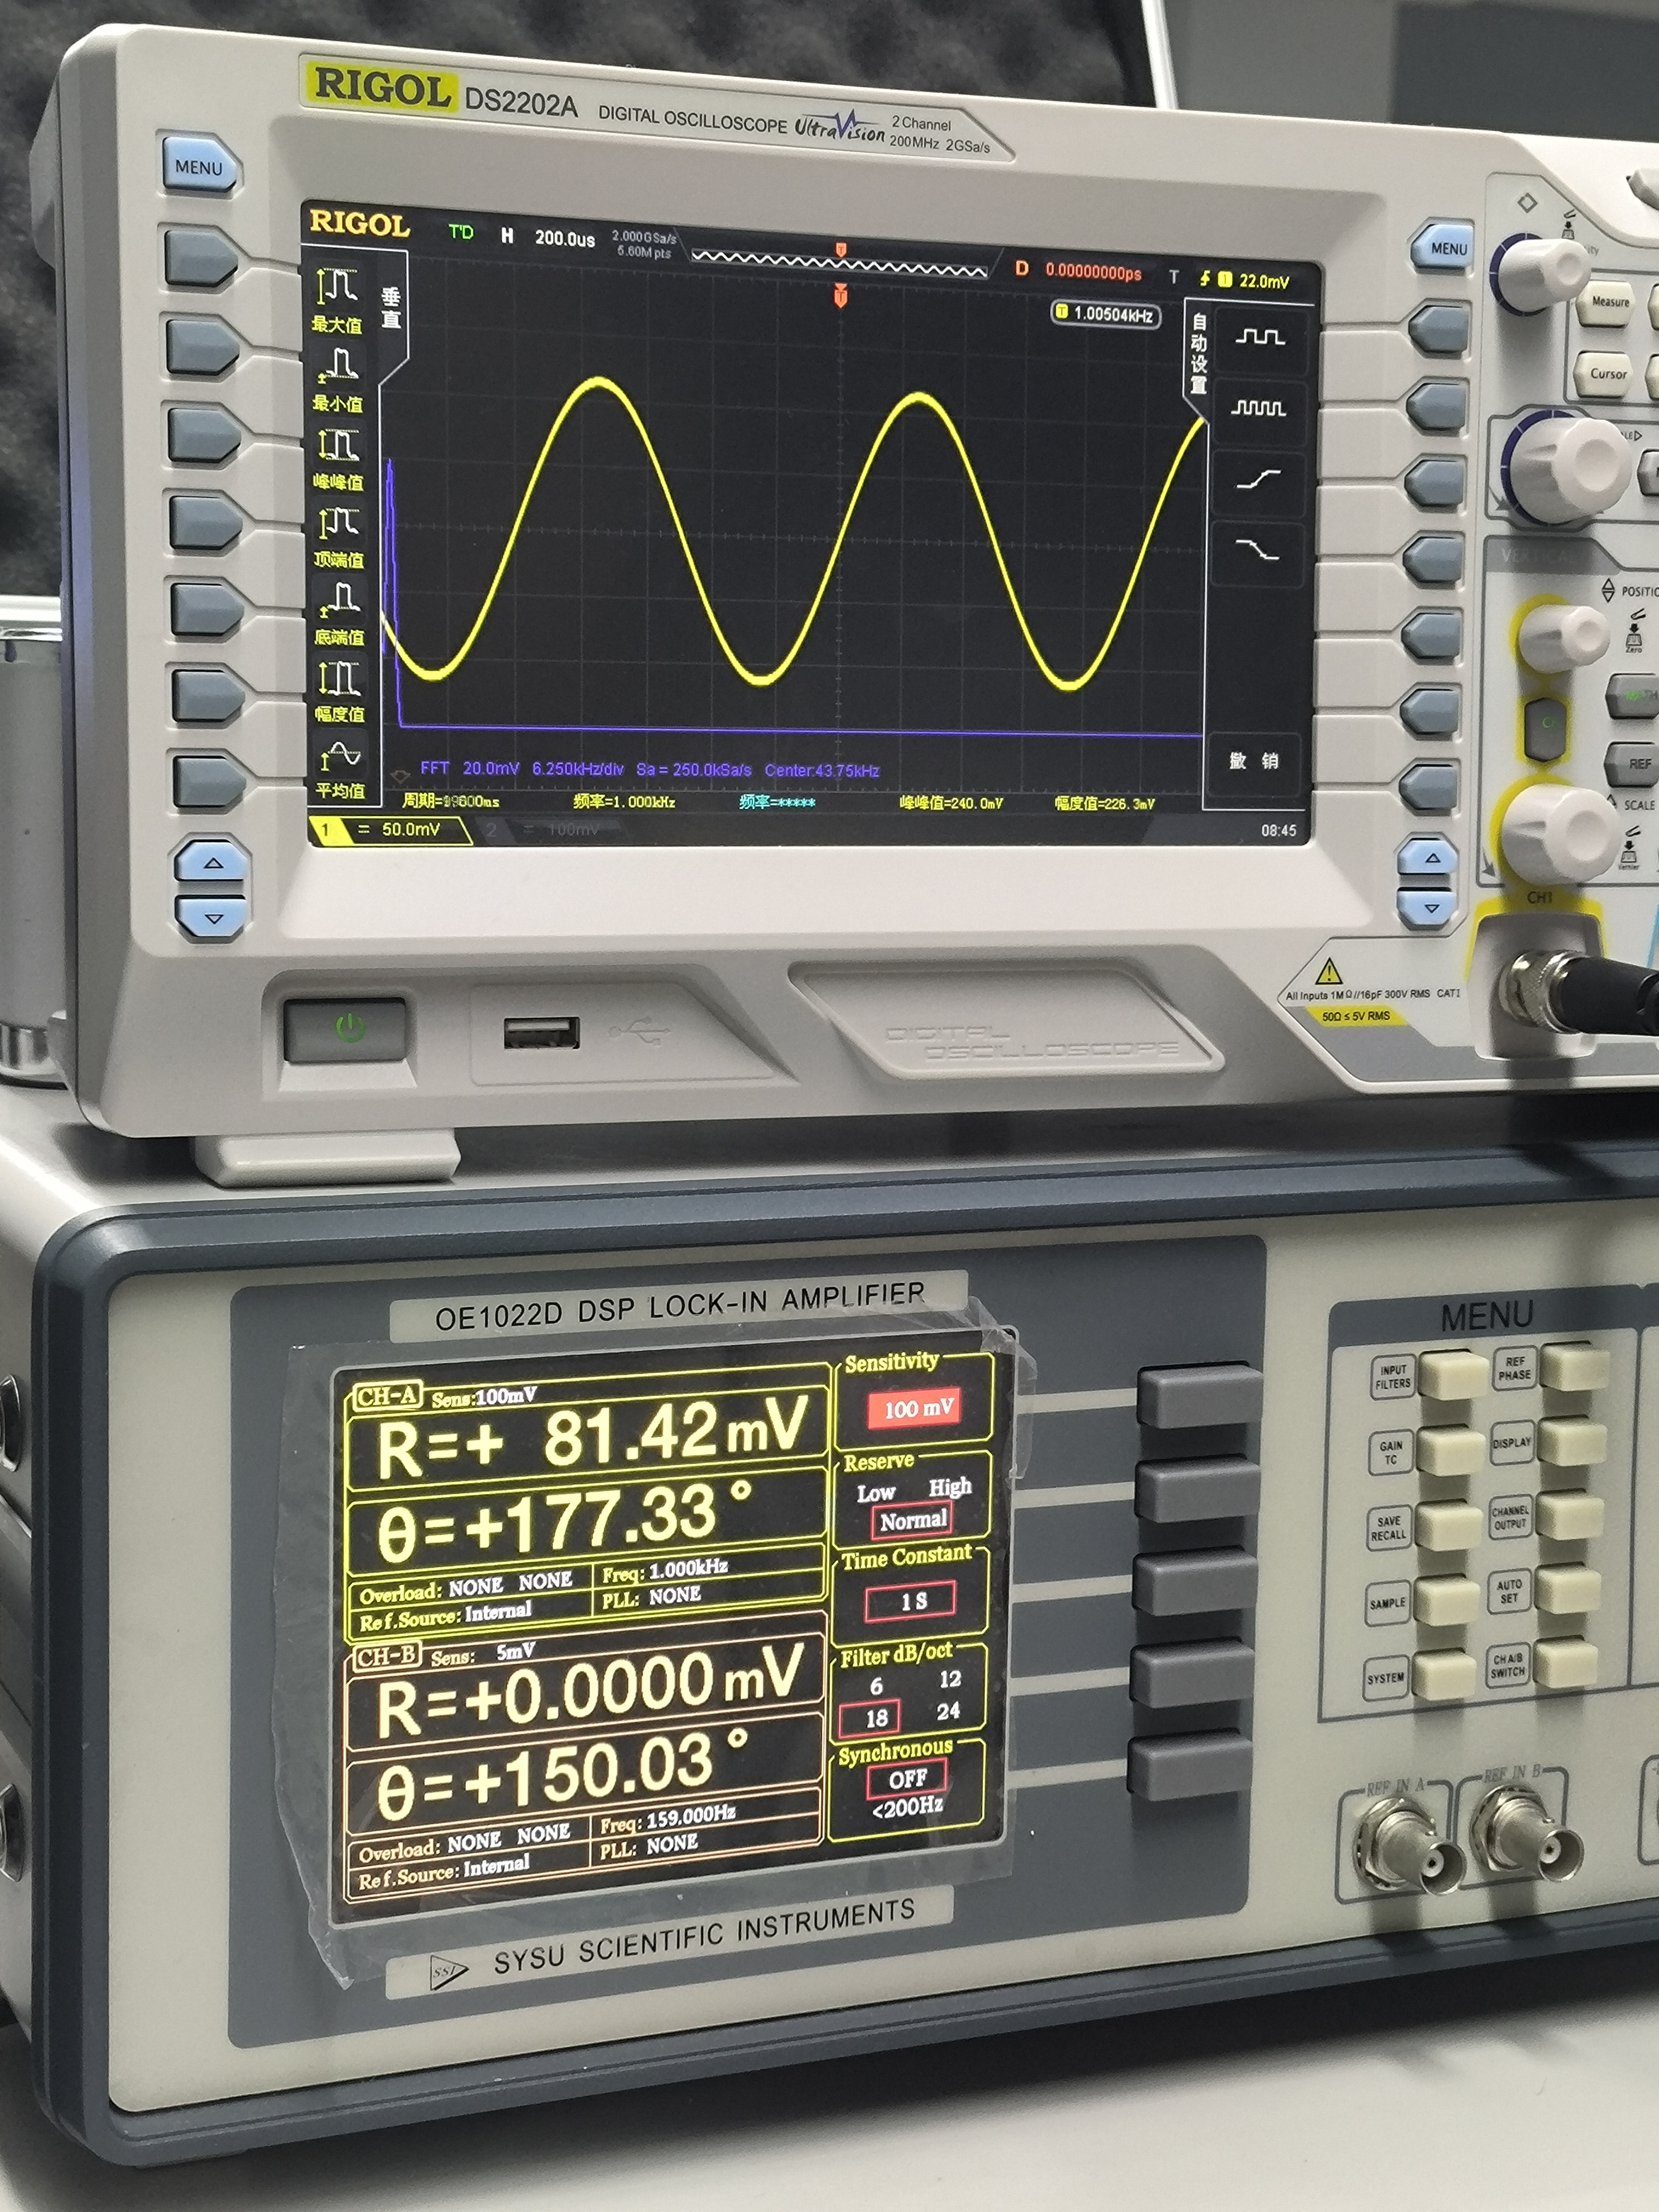
\includegraphics[width=0.5\textwidth]{D1-1-1.jpg}
		\caption{用示波器观察内部信号输出}
		\label{fig:D1-1-1}
	\end{wrapfigure}

	在锁相放大器的“SineOutput”中设置“Voltage = 80mVrms”,频率设置为1kHz,即可通过SINE OUT 功能输出一个正弦信号,如\cref{fig:D1-1-1}所示。

	需要注意,当用三通分信号至示波器时,注意在示波器输入通道设置中选择输入阻抗$1\mathrm{M}\Omega$。通过示波器测量到的信号确实为正弦波,测量信号的峰峰值$V_{pp} = 240.0 \text{mV}$,频率$f = 1.000 \text{kHz}$。

	% 即测量的有效值为$$V_{rms} = \frac{V_{pp}}{2\sqrt{2}} = 84.85 \text{mV}$$ 与设定值$80 \text{mV}$之间有一定误差;



	\clearpage
	\subsubsection*{实验1.2 \quad 测量信号 $R$、$\theta$、$X$以及$Y$值,并验证它们之间的关系}

	在实验一的基础上,用一条BNC-BNC 信号线连接 OE1022 前面板 SINE OUT 输出接口和 SIGNAL IN 的 A/I接口,并设置合适的数字信号发生器输出幅值和量程灵敏度值,确保不会发生前级输出溢出和放大溢出的情况。具体实验时,设置量程灵敏度为100mV。
	
	通过前面板DISPLAY按键,测量实时显示的$R$、$\theta$、$X$、$Y$值,结果如\cref{tbl:D1-2-1}。

	\begin{table}[htbp]
		\centering
		\begin{tabular}{|llll|} 
		\hline
		$R/\text{mV}$  & $X/\text{mV}$   & $Y/\text{mV}$ & $\theta/°$  \\ 
		\hline
		81.43 & -81.34 & 3.79 & 177.33   \\
		\hline
		\end{tabular}
		\caption{测量信号的 $R$、$\theta$、$X$、$Y$值}
		\label{tbl:D1-2-1}
	\end{table}





	\subsubsection*{实验1.3 \quad 相敏检波器工作原理——乘法器}

	将锁相放大器设置为内部参考信号,耦合方式设置为DC,将滤波器带宽调至最大(即$TC = 10 \mu\text{s}, \text{Slope} = 6 \text{dB/cot}$)。设置一个幅值为320mVrms,频率为1kHz的正弦波信号输入锁相放大器,量程灵敏度设置为500mV。
	
	通过示波器观察锁相放大器的模拟输出的$R$信号的波形,如\cref{fig:D1-3-1}所示;同时观察$X$,$Y$信号的波形,如\cref{fig:D1-3-3}所示。

	在相同的陡降(6dB/oct)下,设置不同的时间常数,观察其对$X$、$Y$信号平均值的影响,结果如\cref{tbl:D1-3-1}所示。



	\begin{figure}[htbp]
		\centering
		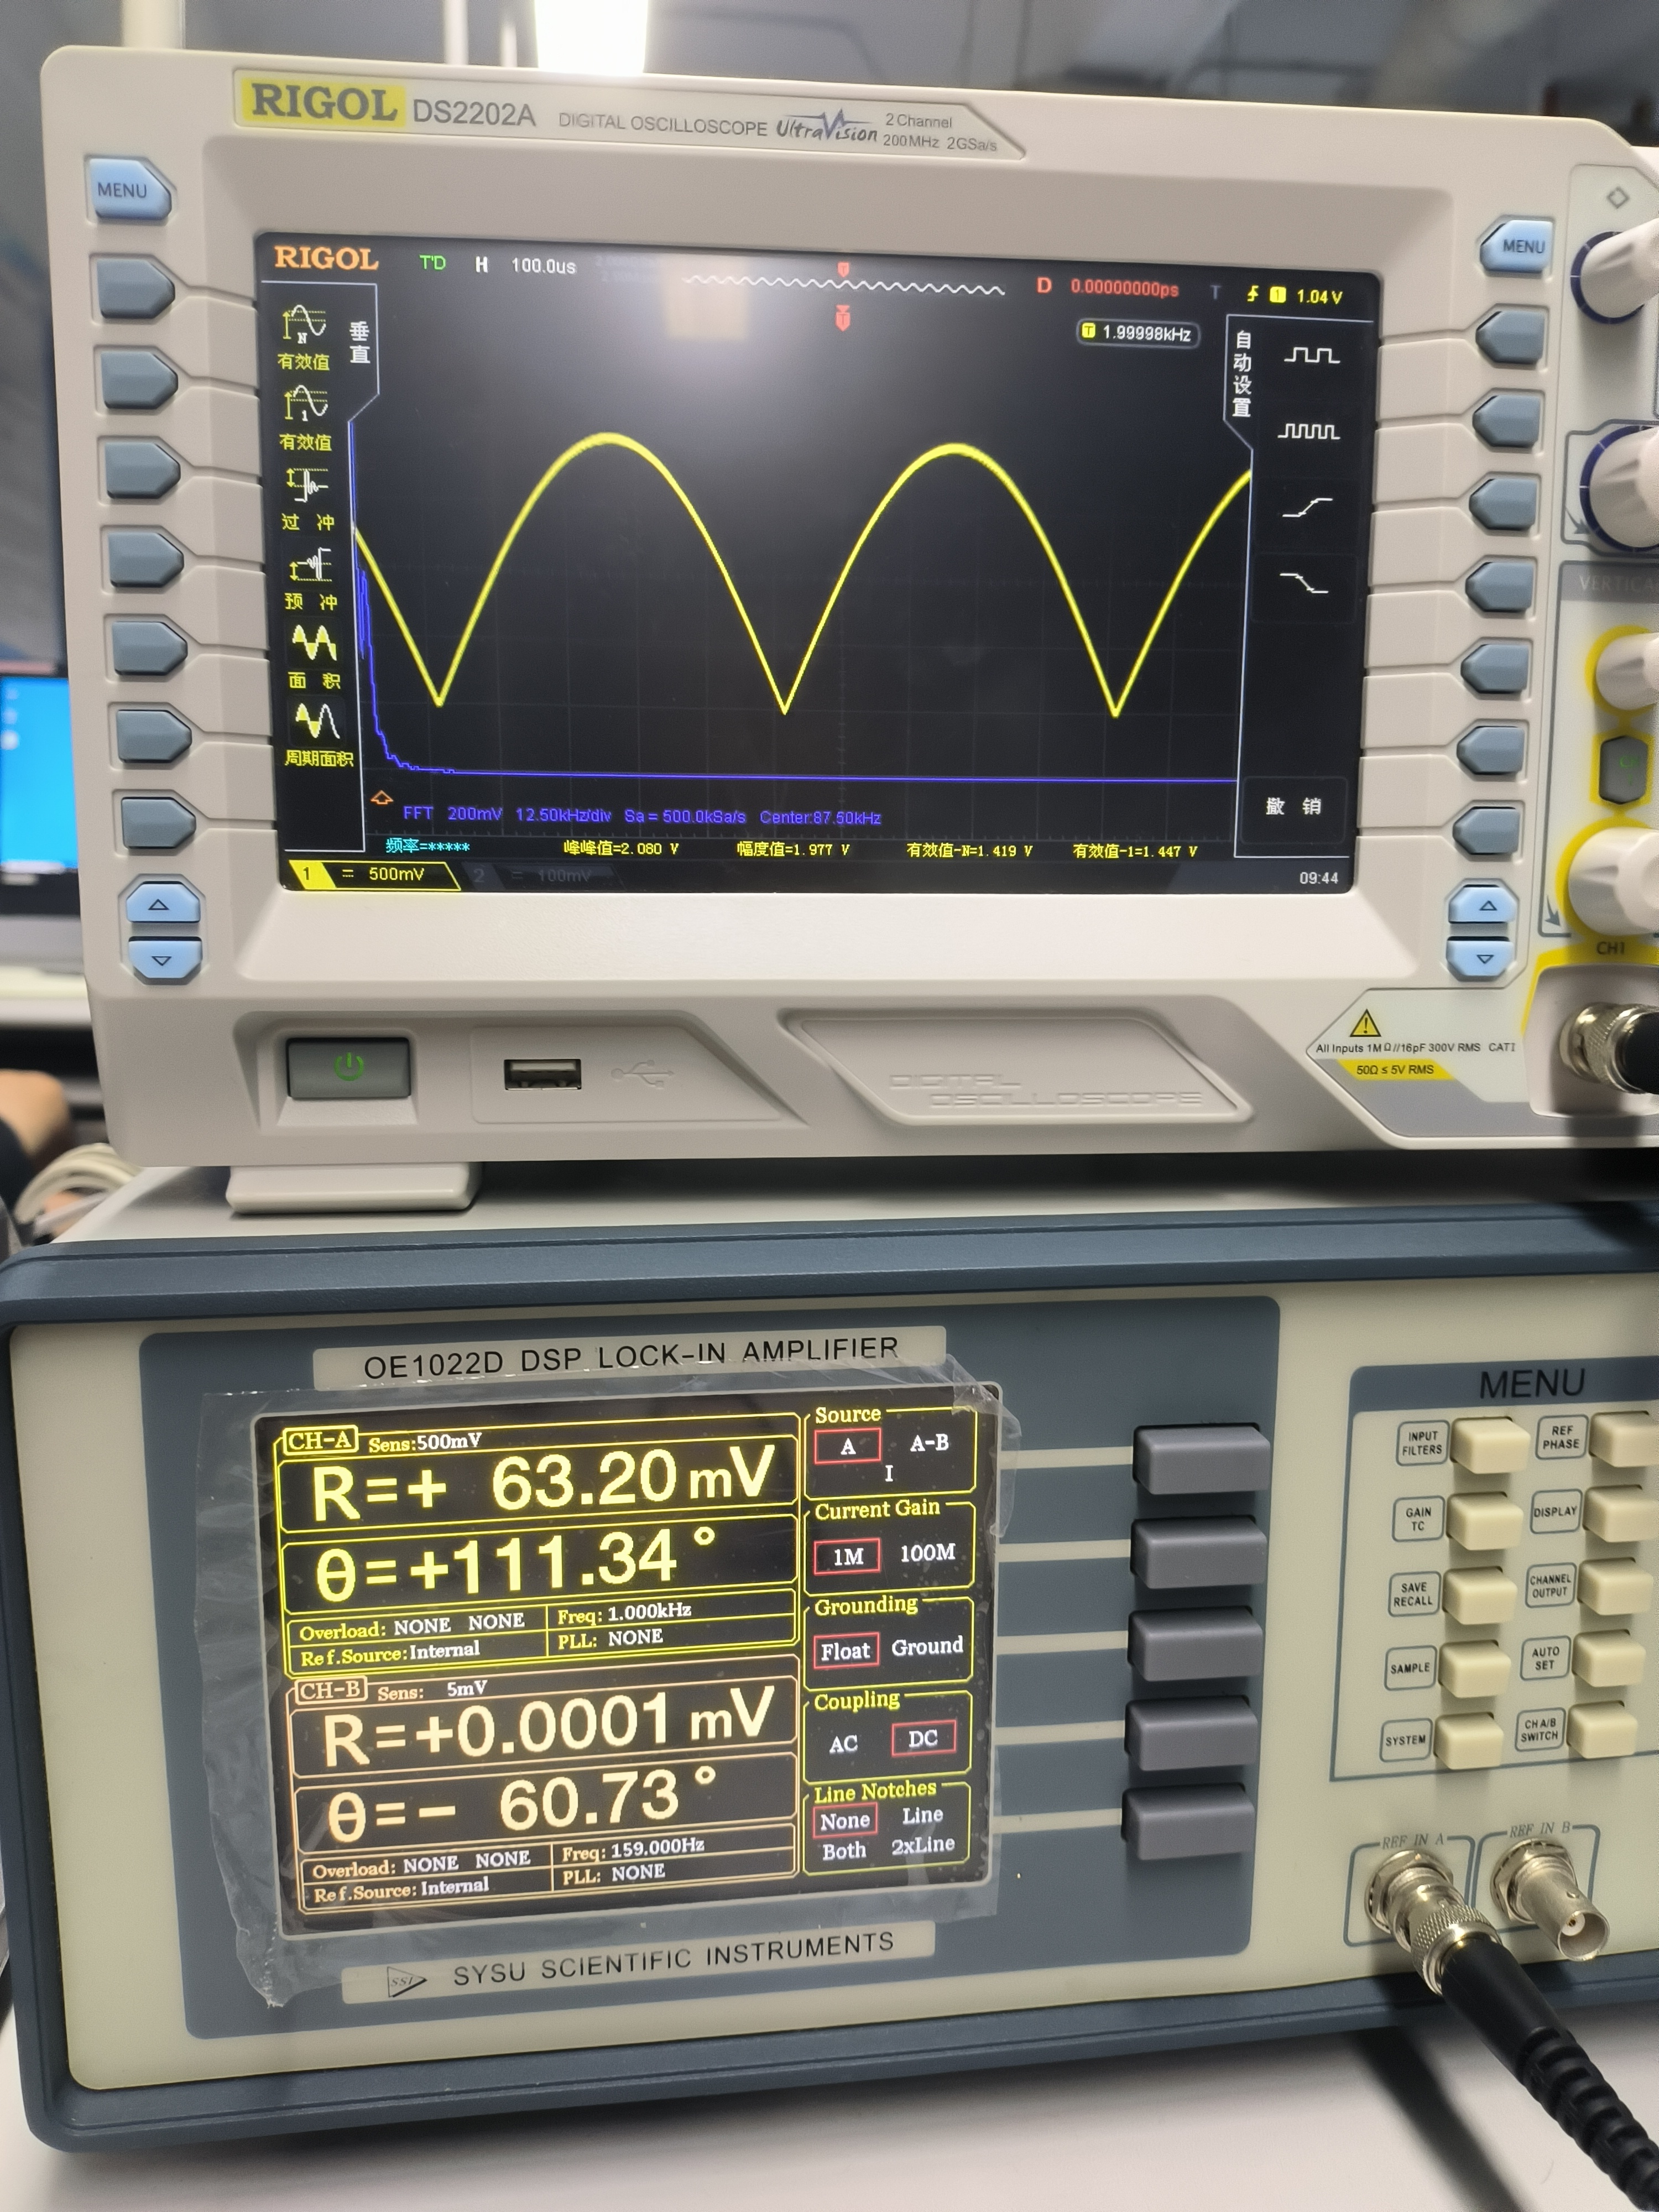
\includegraphics[width=0.45\textwidth]{D1-3-1.jpg}
		\caption{乘法器输出的$R$的图像}
		\label{fig:D1-3-1}
	\end{figure}


	\begin{figure}[htbp]
		\centering
		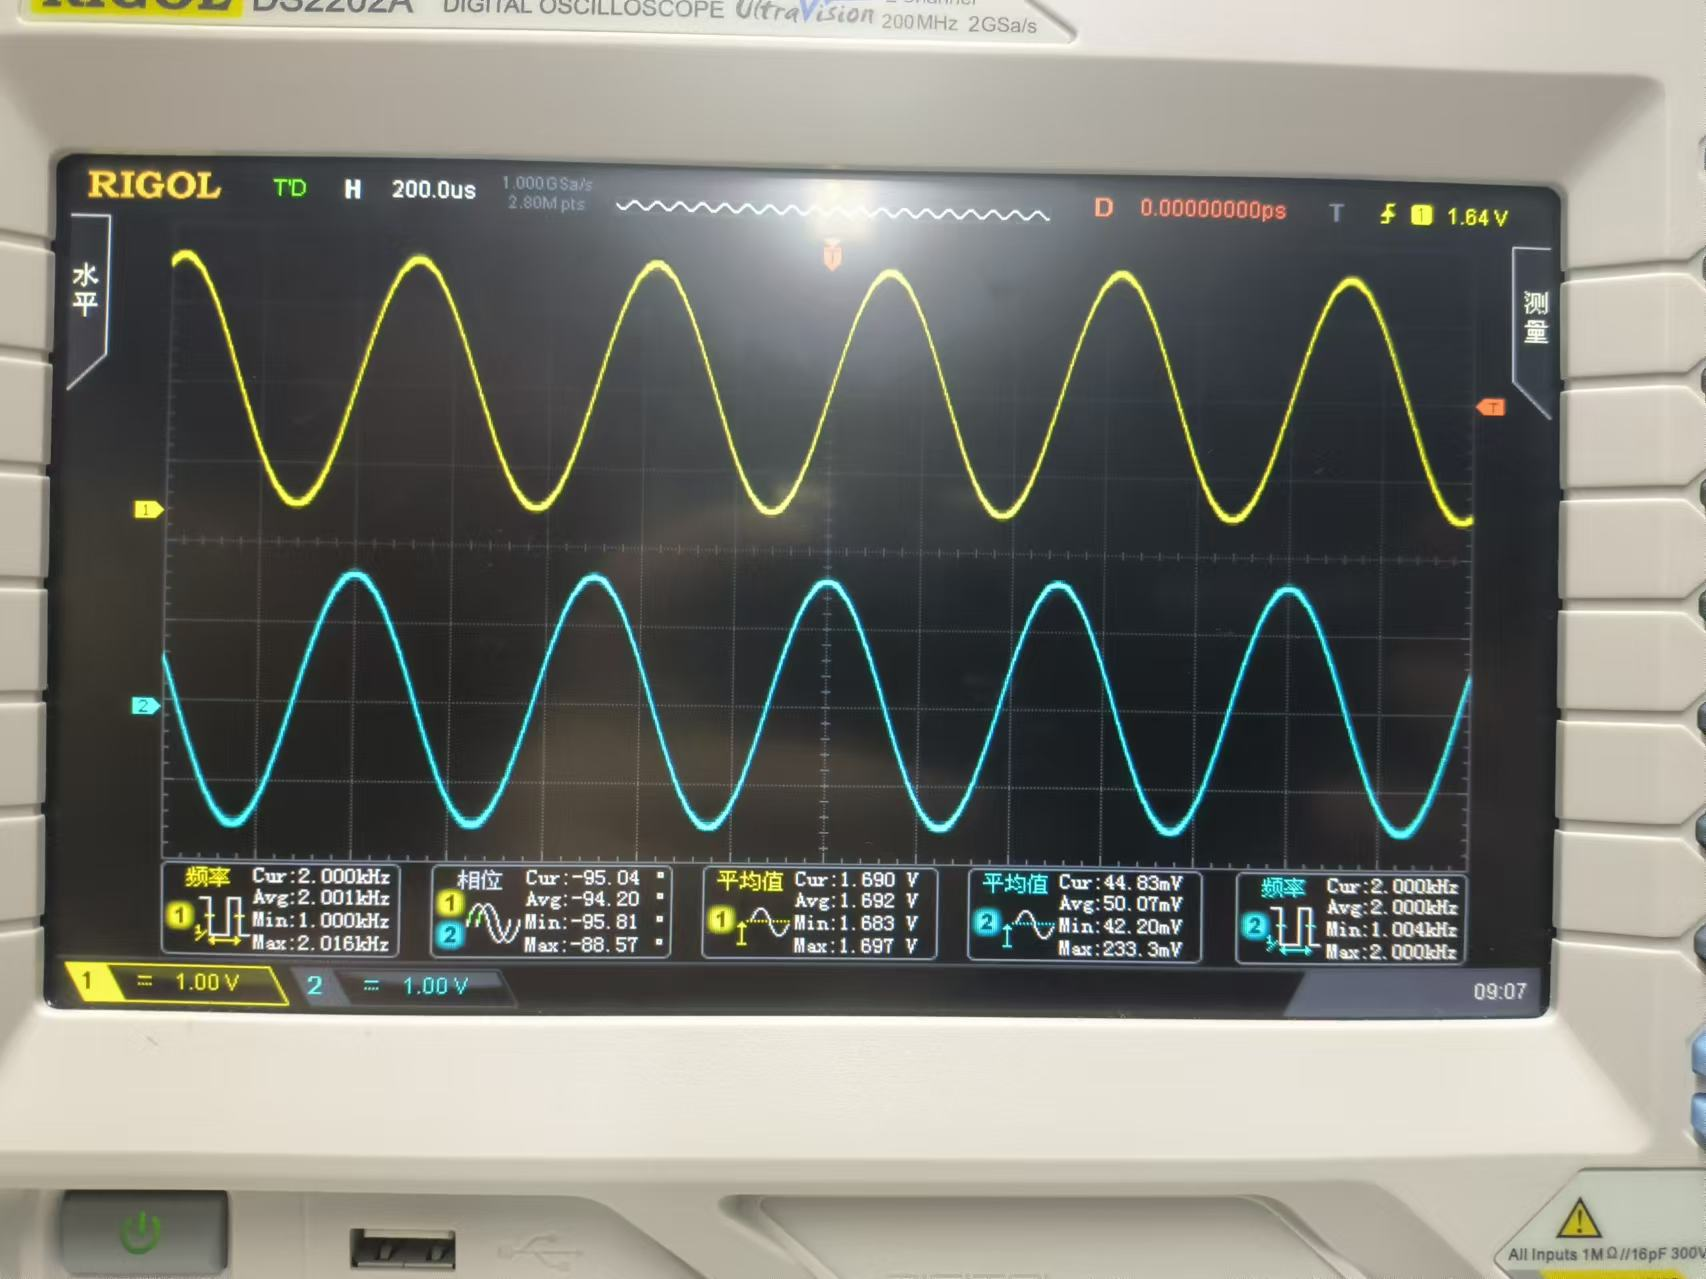
\includegraphics[width=0.6\textwidth]{D1-3-3.jpg}
		\caption{乘法器输出的$X$,$Y$的图像}
		\label{fig:D1-3-3}
	\end{figure}


	\begin{table}
		\centering
		\begin{tabular}{|c|cc|} 
		\hline
		\diagbox{时间常数}{平均值}{信号} & $X/ \mathrm{mV}$     & $Y/ \mathrm{mV}$      \\ 
		\hline
		10$\mu$s                           & 1.692 & 50.07  \\
		100us                              & 1.692 & 53.59  \\
		1ms                                & 1.690 & 51.13  \\
		10ms                               & 1.690 & 48.65  \\
		100ms                              & 1.692 & 49.82  \\
		1s                                 & 1.691 & 49.47  \\
		\hline
		\end{tabular}
		\caption{相同的陡降、不同的时间常数对$X$、$Y$信号平均值的影响}
		\label{tbl:D1-3-1}
	\end{table}






	\subsubsection*{实验1.4 \quad 相敏检波器工作原理——乘法器+低通滤波器}

	对锁相放大器的滤波器设置不同的时间常数和陡降,通过示波器观察锁相放大器的输入信号波形、乘法器输出的$R$,$X$,$Y$波形,同时记录锁相放大器的$R$,$X$,$Y$读数,如\cref{tbl:D1-4-1}所示。



	不断增大陡降,观察输出的滤波波形,图像如\cref{fig:D1-4-1-1}、\cref{fig:D1-4-1-2}、\cref{fig:D1-4-1-3}、\cref{fig:D1-4-1-4}所示

	\begin{table}[htbp]
		\centering
		\begin{tblr}{
		  cells = {c},
		  cell{1}{1} = {r=2}{},
		  cell{1}{2} = {r=2}{},
		  cell{1}{3} = {c=3}{},
		  cell{1}{6} = {c=3}{},
		  cell{3}{1} = {r=6}{},
		  vline{1,2,3,6,9} = {1,2}{},
		%   vline{1,2,3,6,9} = {2}{},
		%   vline{1-3,9} = {3}{},
		  vline{1,2,3,6,9} = {3-8}{},
		  hline{1,3,9} = {-}{},
		  hline{2} = {3-8}{},
		}
		陡降(dB/oct) & 时间常数   & 示波器读数  &         &         & 锁相放大器读数 &         &        \\
		   &        & $R$      & $X$       & $Y$       & $R$       & $X$       & $Y$      \\
		6  & 10$\mu$s  &        &         &         &         &         &        \\
		   & 100$\mu$s & 2.11V  & 2.17V   & 2.15V   & 55.0mV  & 50.0mV  & 3.0mV  \\
		   & 1ms    & 278mV  & 222.0mV & 280.0mV & 50.0mV  & 49.0mV  & 2.0mV  \\
		   & 10ms   & 28.0mV & 27.0mV  & 28.0mV  & 50.0mV  & 50.0mV  & 1.6mV  \\
		   & 100ms  & 5V     & 5V      & 160mV   & 50.16mV & 50.13mV & 1.67mV \\
		   & 1s     & 5.04V  & 5.03mV  & 158mV   & 50.16mV & 50.13mV & 1.67mV 
		\end{tblr}
		\caption{不同时间常数下的示波器和锁相放大器读数}
		\label{tbl:D1-4-1}
	\end{table}


	\begin{figure}[htbp]
		\centering
		% 第一行左图
		\begin{minipage}[b]{0.45\textwidth}
			\centering
			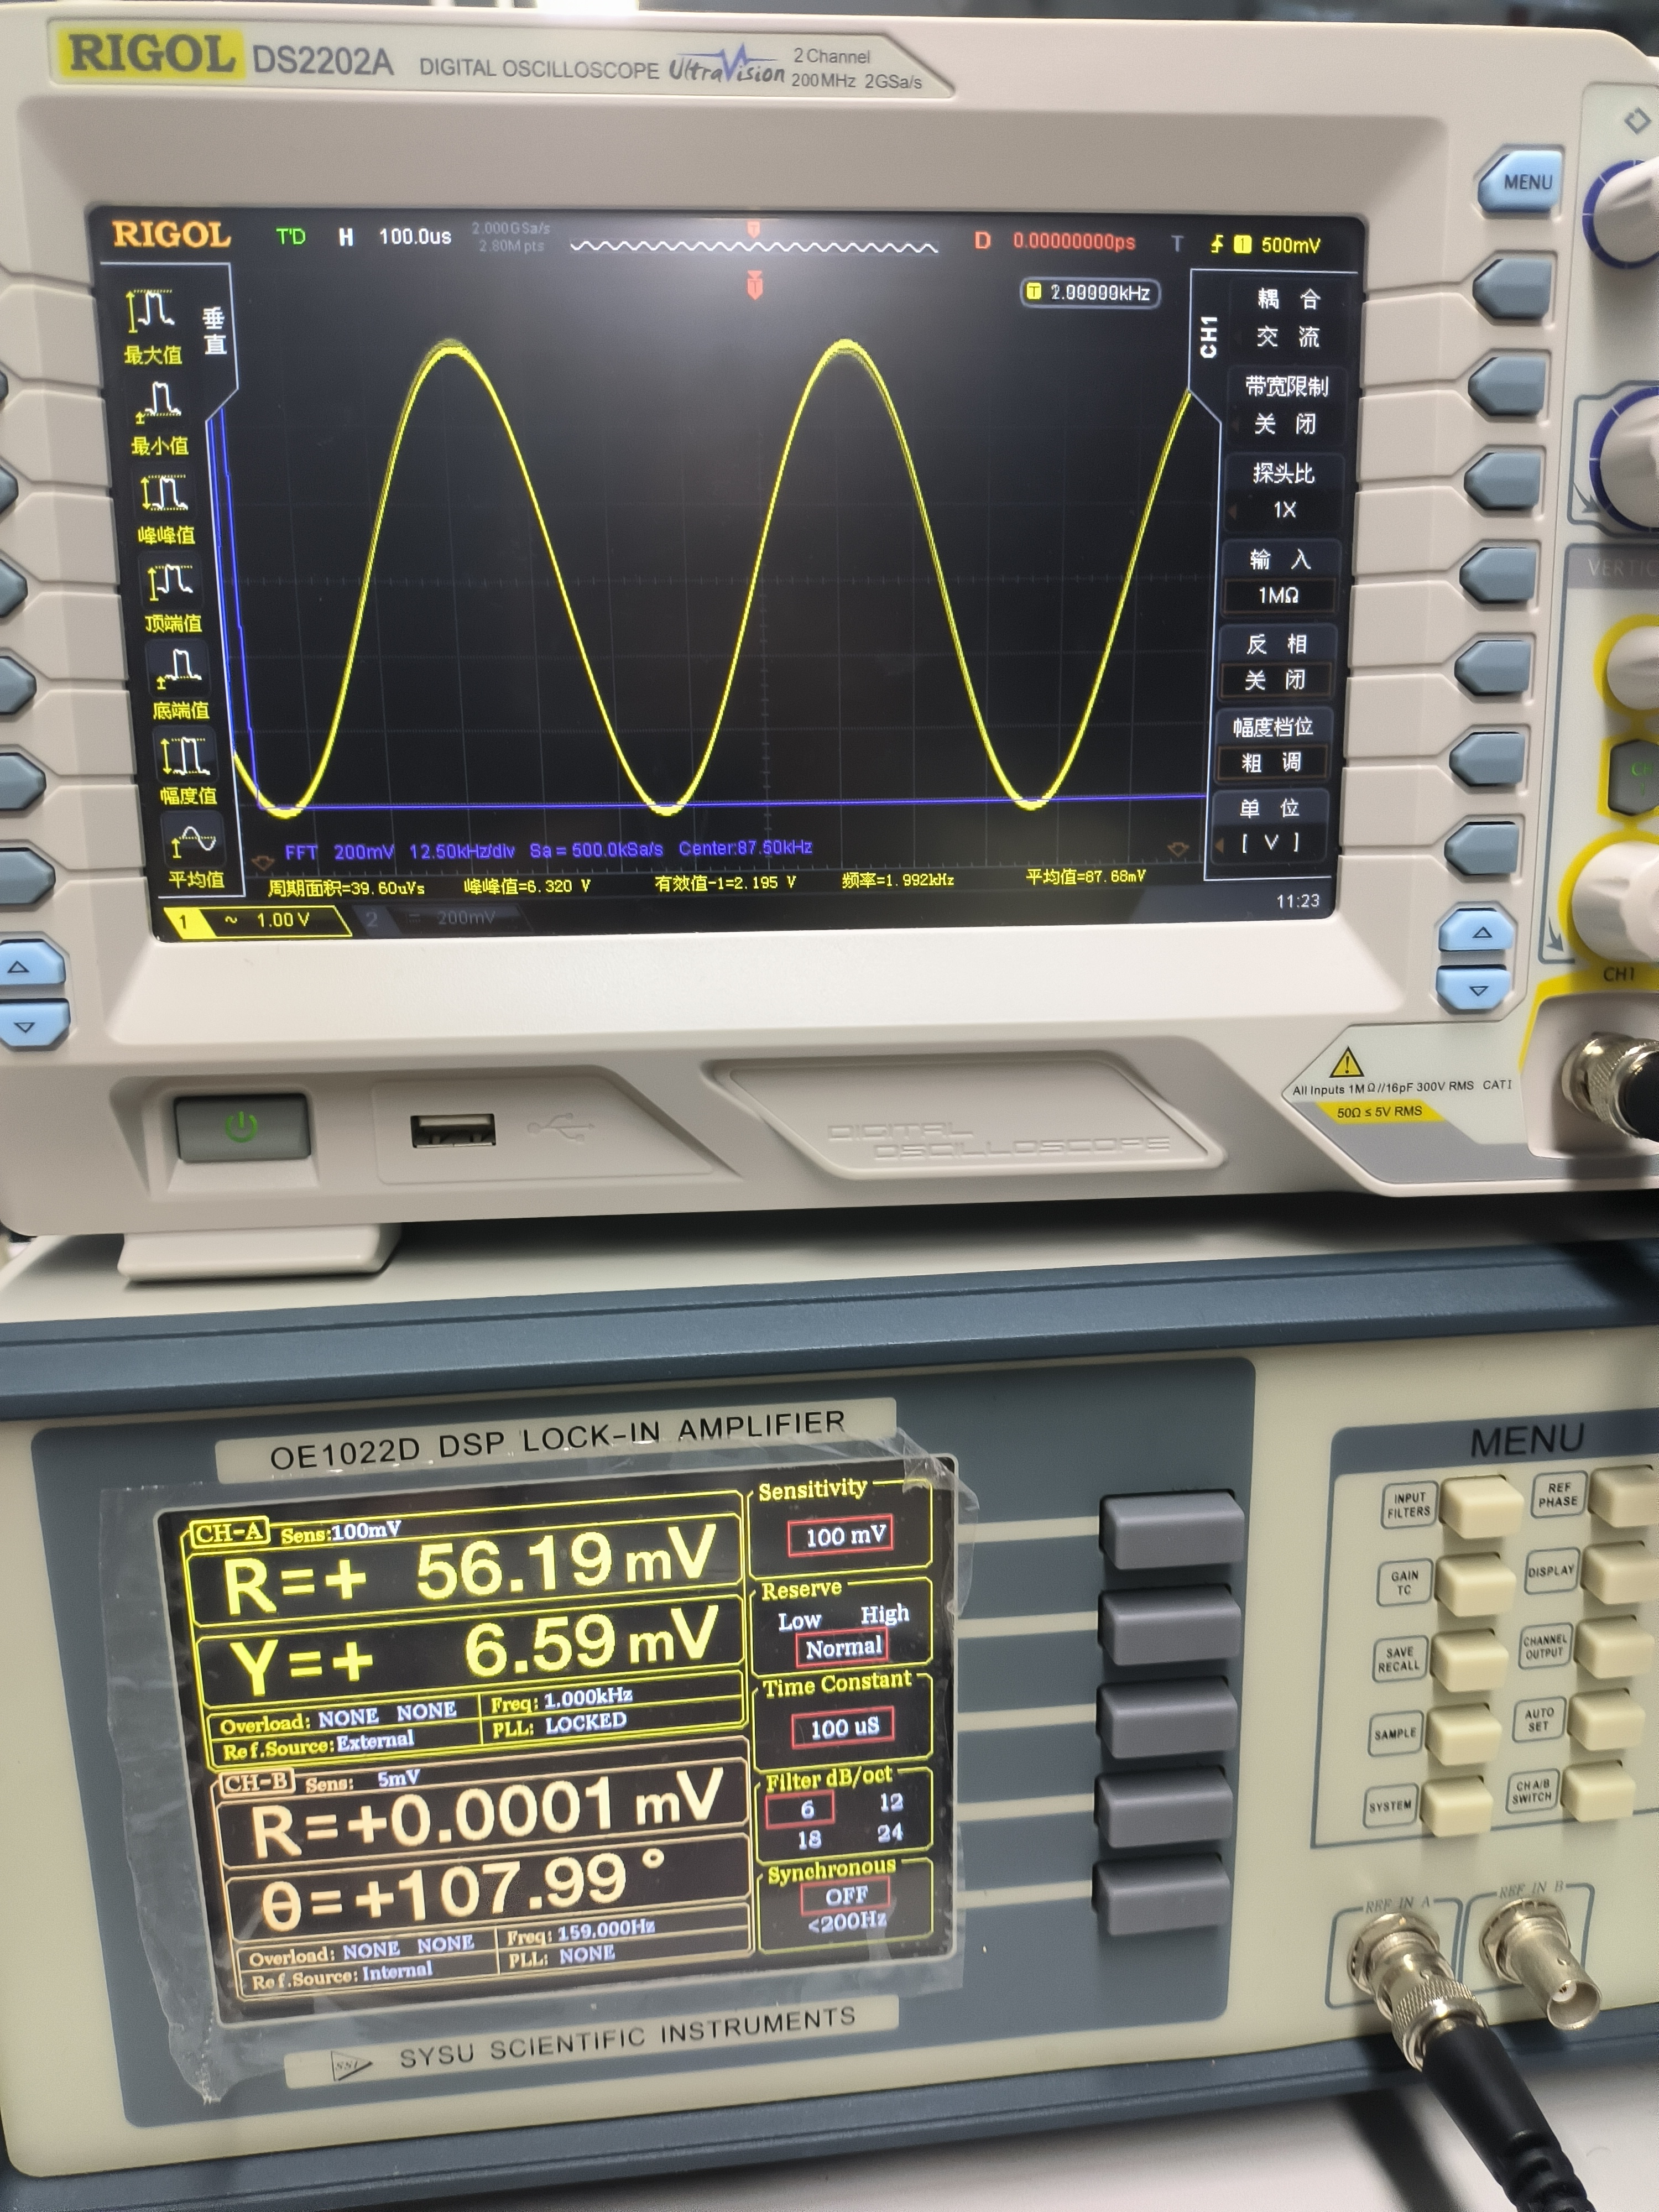
\includegraphics[width=\textwidth]{APL1_1_question8_slope6.jpg} % 替换为你的图片路径
			\caption{$Slope = 6 \mathrm{dB/oct}$}
			\label{fig:D1-4-1-1}
		\end{minipage}
		\hspace{0.05\textwidth} % 两列之间的水平间距
		% 第一行右图
		\begin{minipage}[b]{0.45\textwidth}
			\centering
			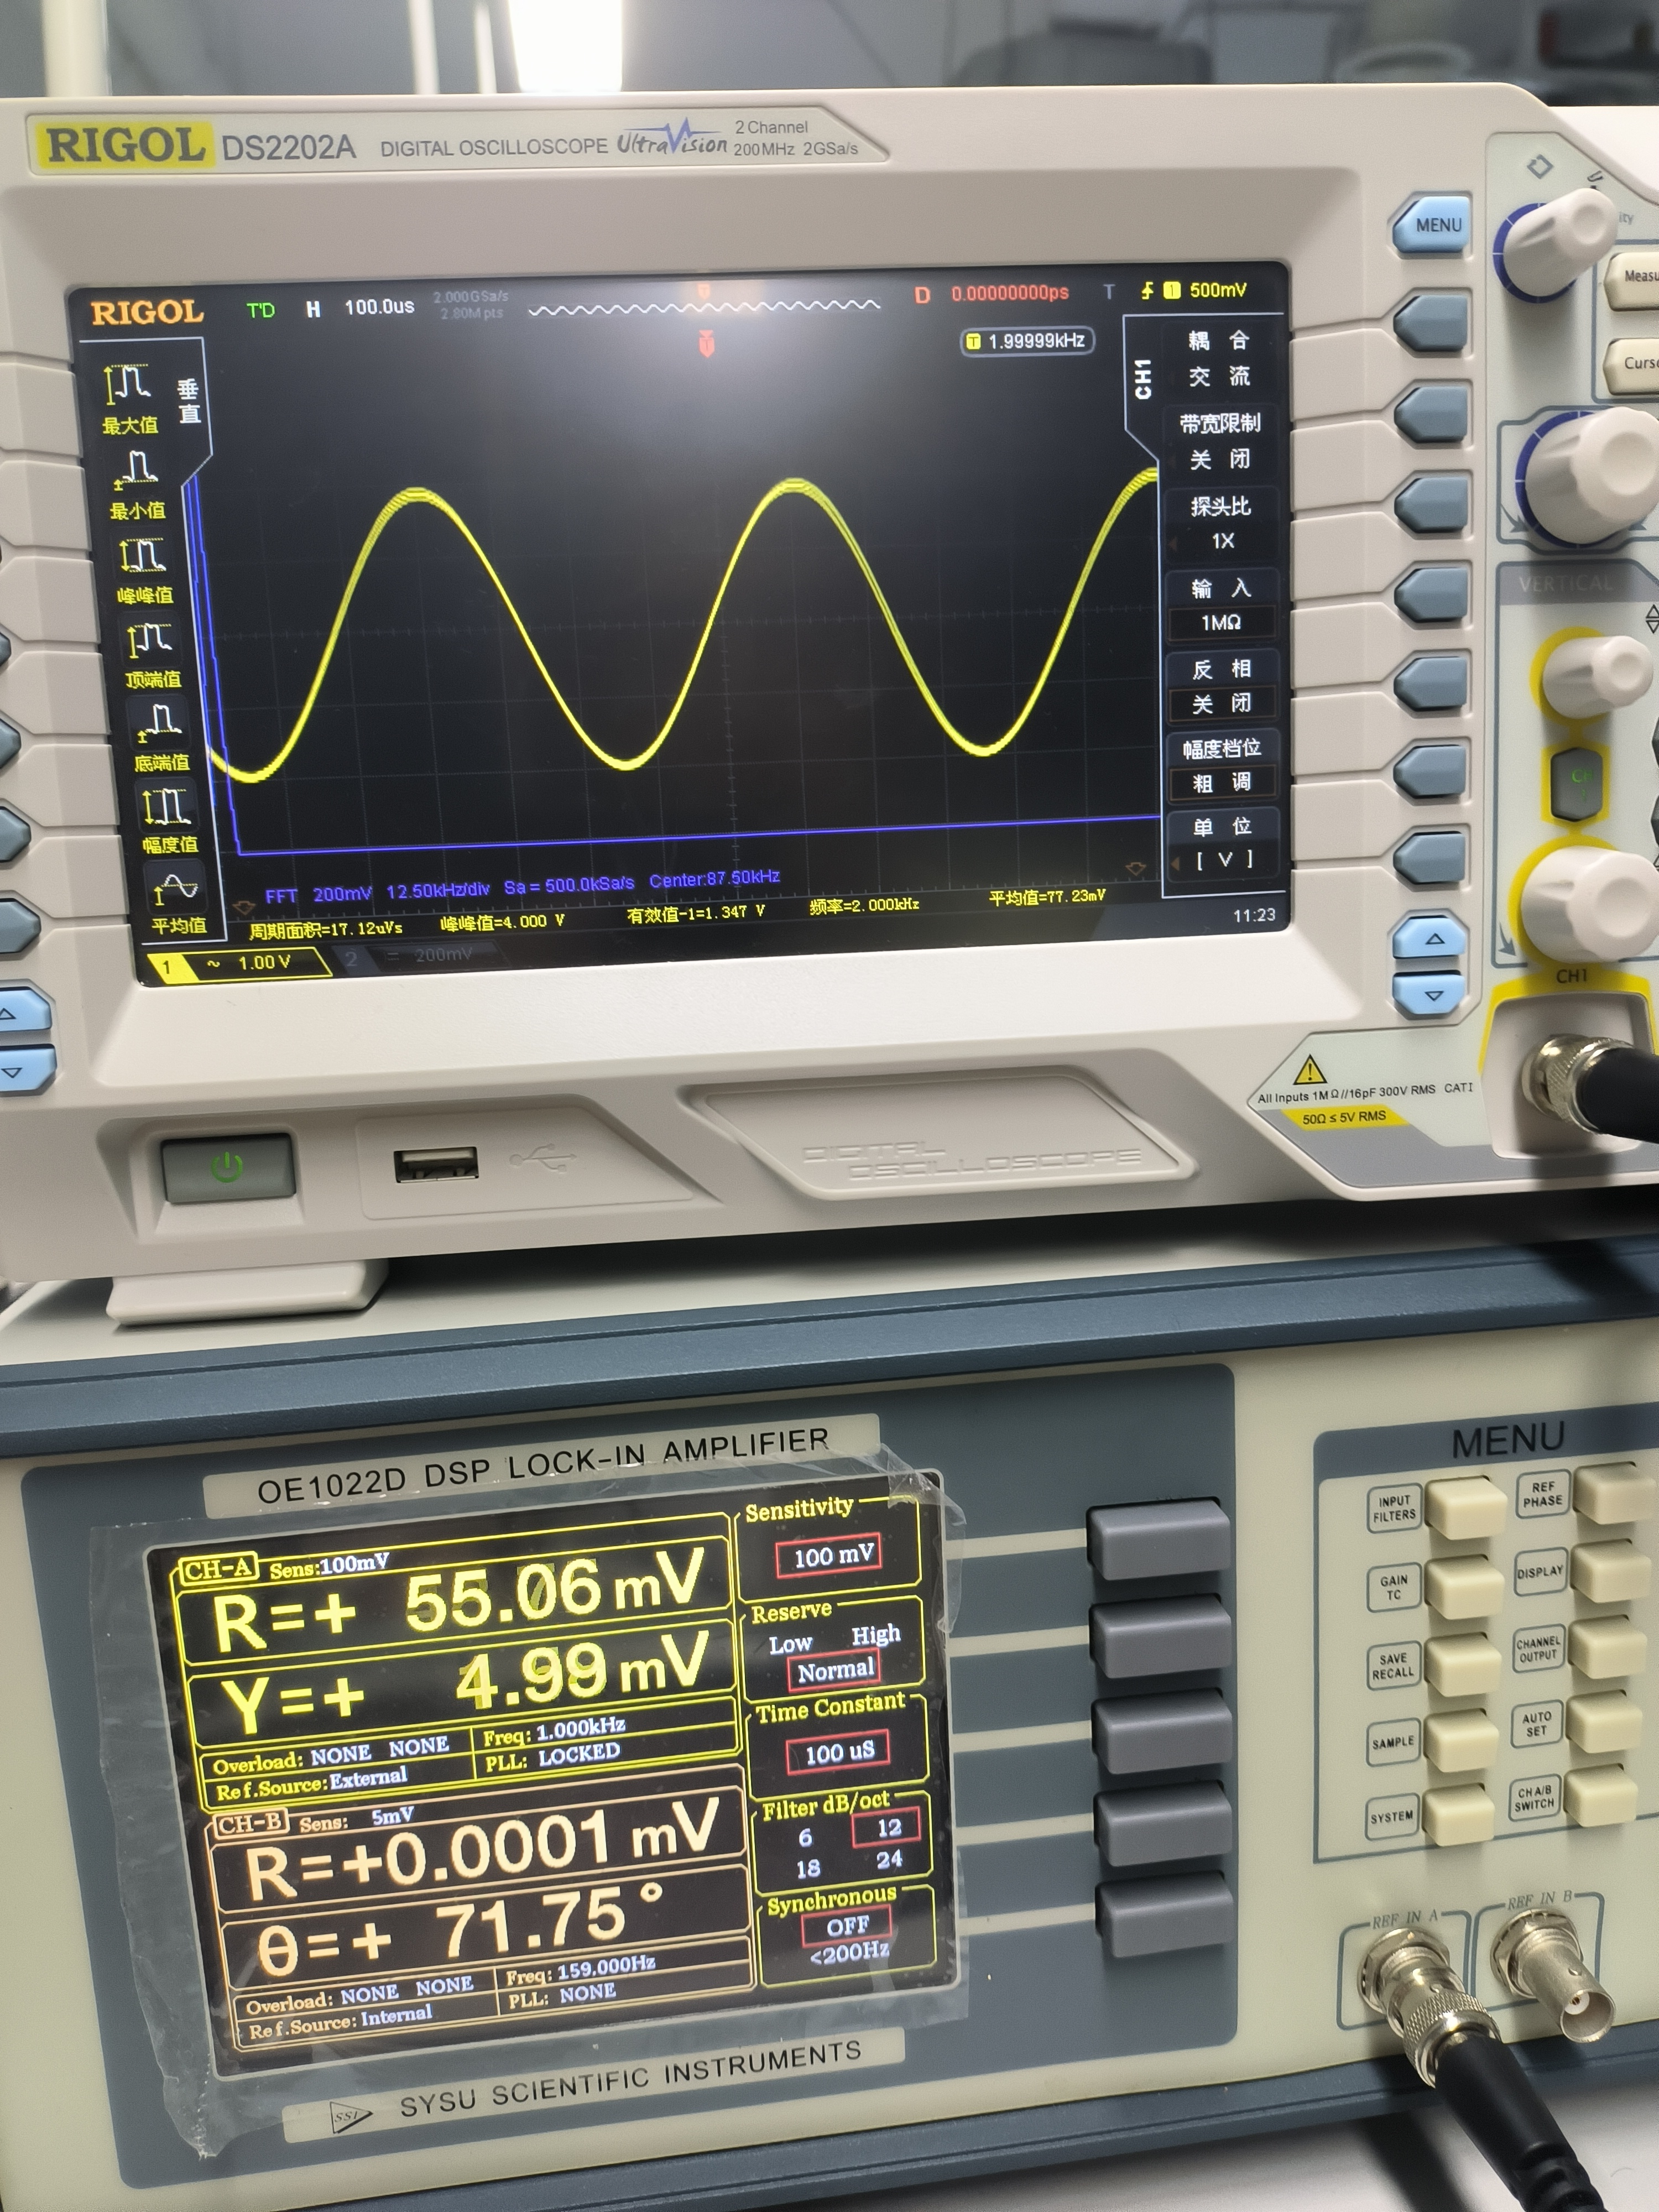
\includegraphics[width=\textwidth]{APL1_1_question8_slope12.jpg} % 替换为你的图片路径
			\caption{$Slope = 12 \mathrm{dB/oct}$}
			\label{fig:D1-4-1-2}
		\end{minipage}
		
		\vspace{0.01\textwidth} % 两行之间的垂直间距
	
		% 第二行左图
		\begin{minipage}[b]{0.45\textwidth}
			\centering
			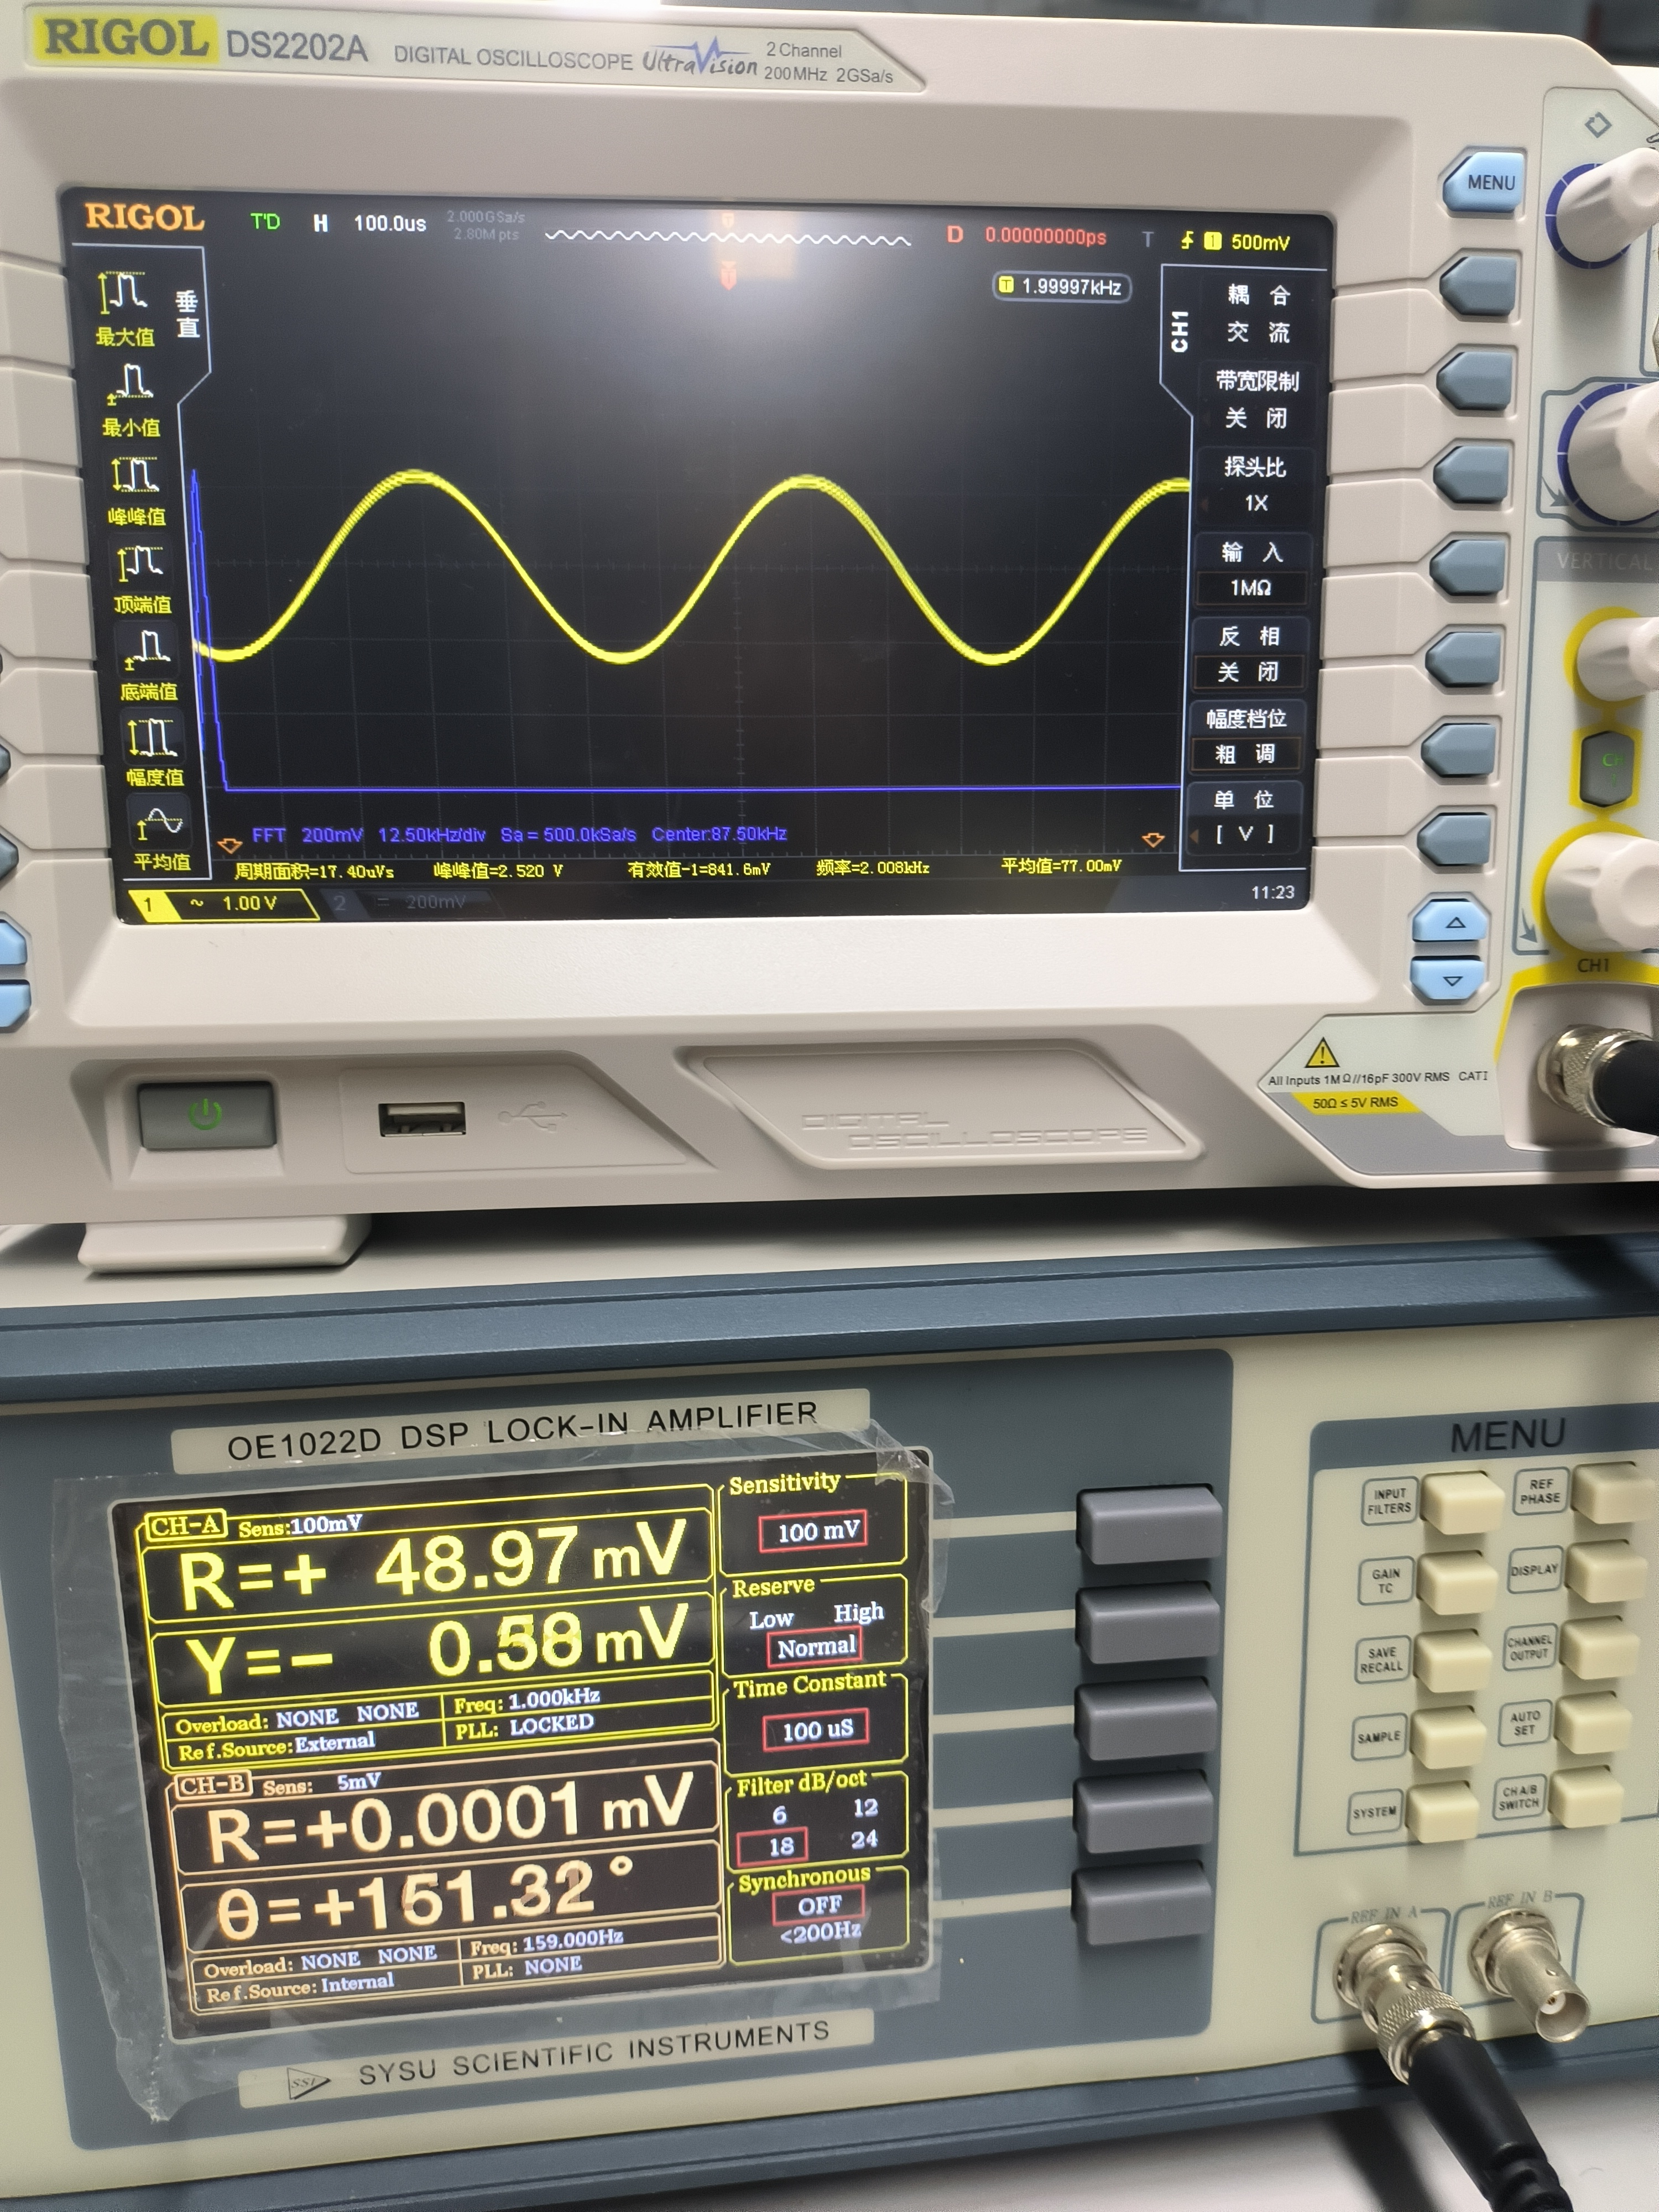
\includegraphics[width=\textwidth]{APL1_1_question8_slope18.jpg} % 替换为你的图片路径
			\caption{$Slope = 18 \mathrm{dB/oct}$}
			\label{fig:D1-4-1-3}
		\end{minipage}
		\hspace{0.05\textwidth} % 两列之间的水平间距
		% 第二行右图
		\begin{minipage}[b]{0.45\textwidth}
			\centering
			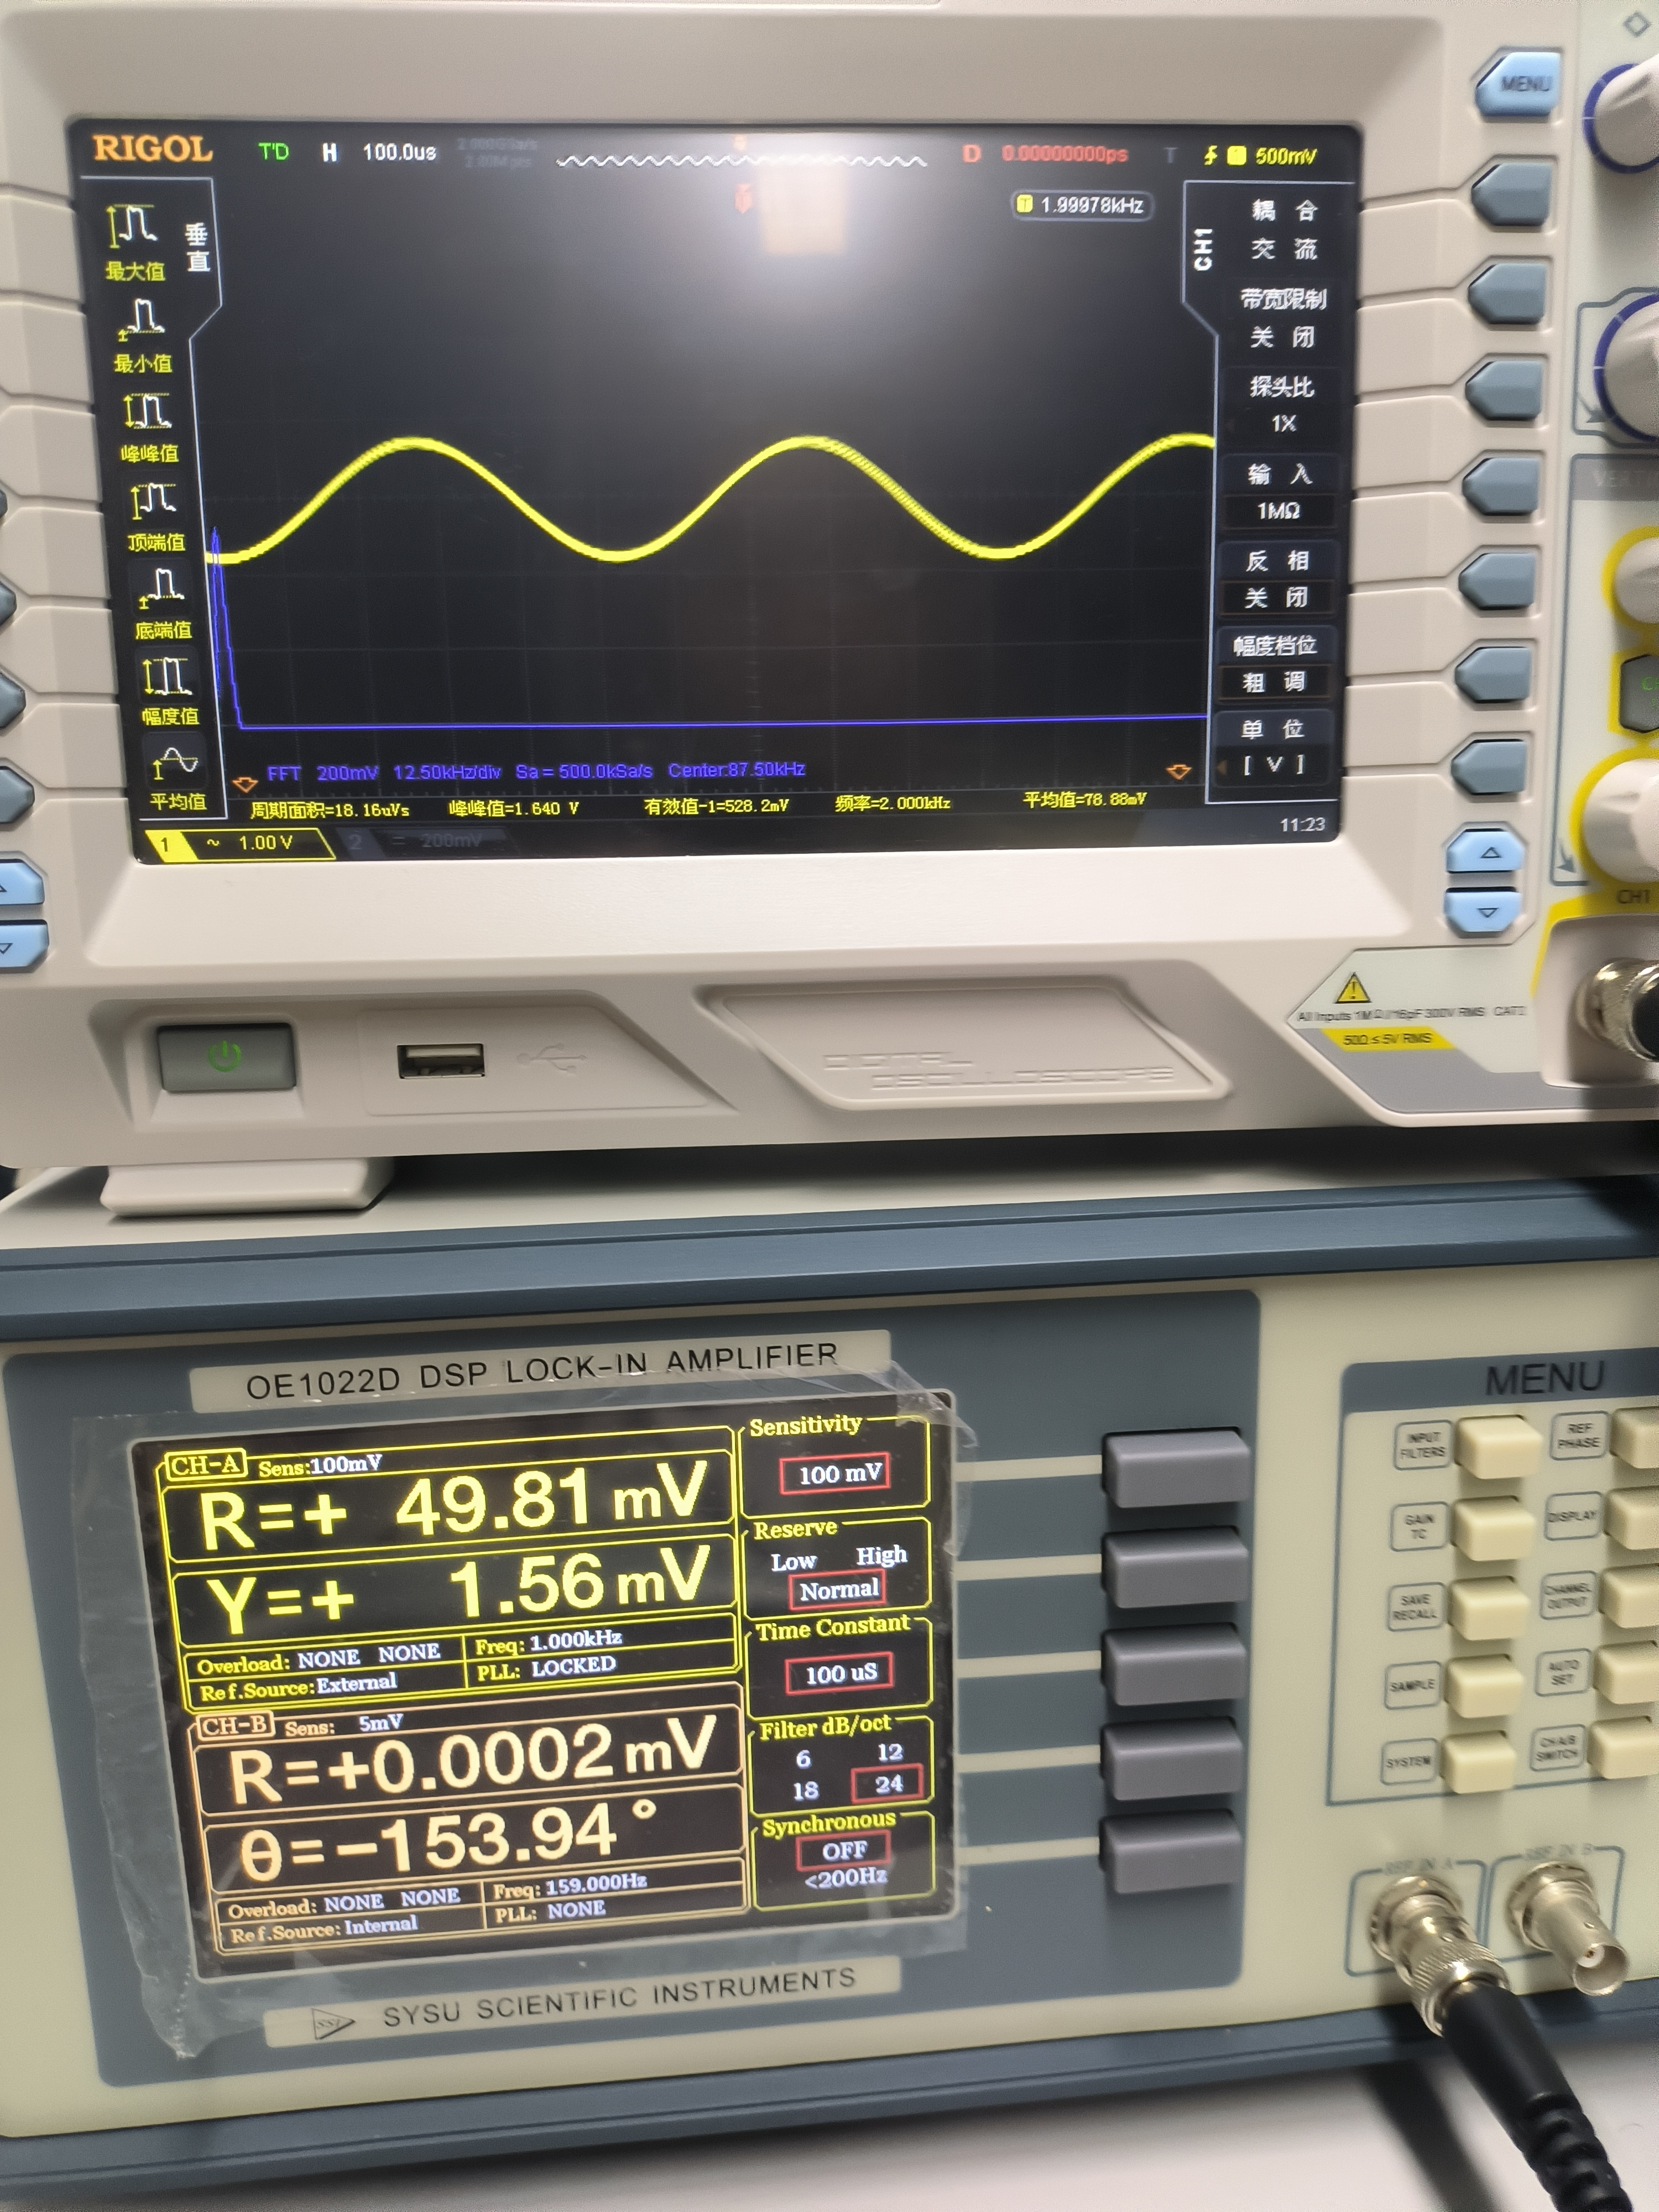
\includegraphics[width=\textwidth]{APL1_1_question8_slope24.jpg} % 替换为你的图片路径
			\caption{$Slope = 24 \mathrm{dB/oct}$}
			\label{fig:D1-4-1-4}
		\end{minipage}
		\caption*{不同陡降的滤波效果}
		\label{fig:D1-4-1}
	\end{figure}









	\clearpage
	\subsubsection*{实验1.8 \quad 强噪声背景下的弱信号检测}

	\begin{wrapfigure}{l}{0.5\textwidth}
		\centering
		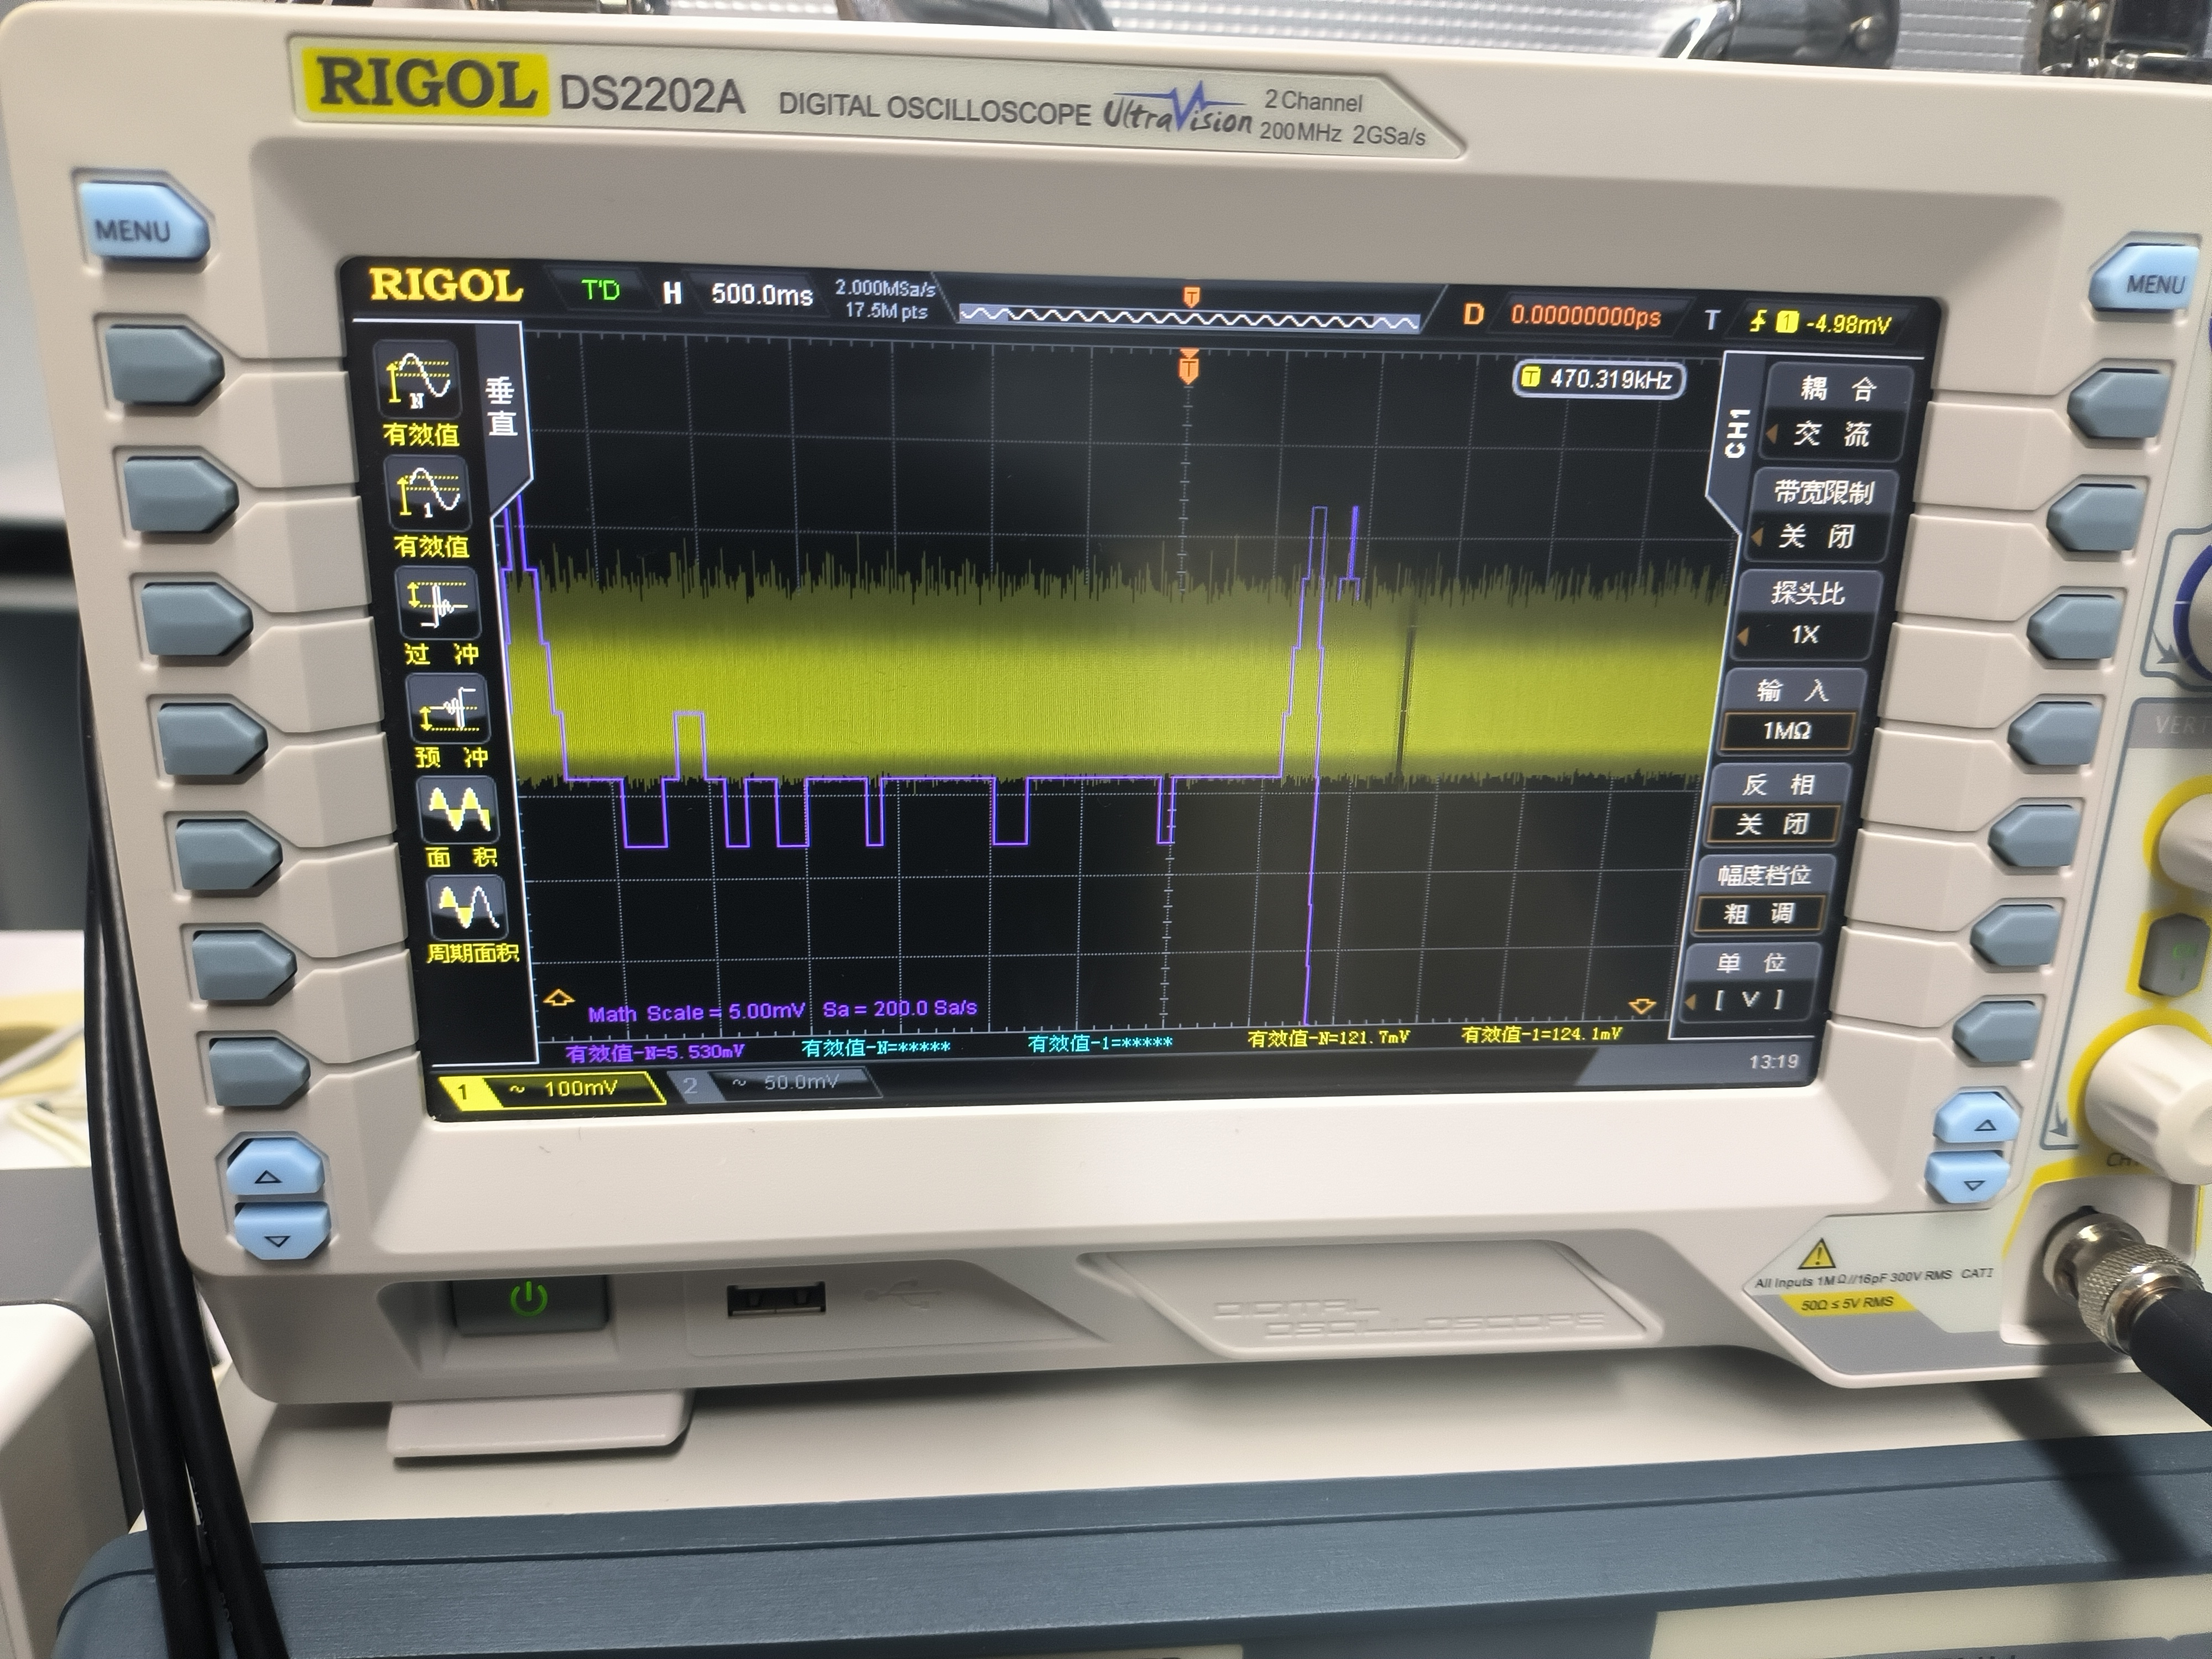
\includegraphics[width=0.5\textwidth]{D1-8-1.jpg}
		\caption{噪声发生器的噪声信号测量}
		\label{fig:D1-8-1}
	\end{wrapfigure}

	通过白噪声发生器产生约100mVrms的白噪声,将其与不同幅值的正弦信号相加,得到不同信噪比的待测信号。
	
	实验过程中,首先测量噪声发生器的噪声信号有效值,通过拉长时间轴的方法,让噪声幅值在长时间下取平均,使有效值的数值稳定,如\cref{fig:D1-8-1}所示。

	然后基于测量得到的噪声有效值,设置不同的信号幅值,得到不同的输入信号信噪比。信噪比为0的情况,即设置正弦波幅值$V_{in} = V_{noise}$;信噪比-30的情况,即通过理论计算得到,在噪声有效值一定的情况下,所需的正弦波幅值;信噪比-80的情况,可通过噪声发生器的衰减功能直接在信噪比为0的情况的基础上得到。测量数据如\cref{tbl:D1-8-1}所示。




	% \begin{figure}[htbp]
	% 	\centering
	% 	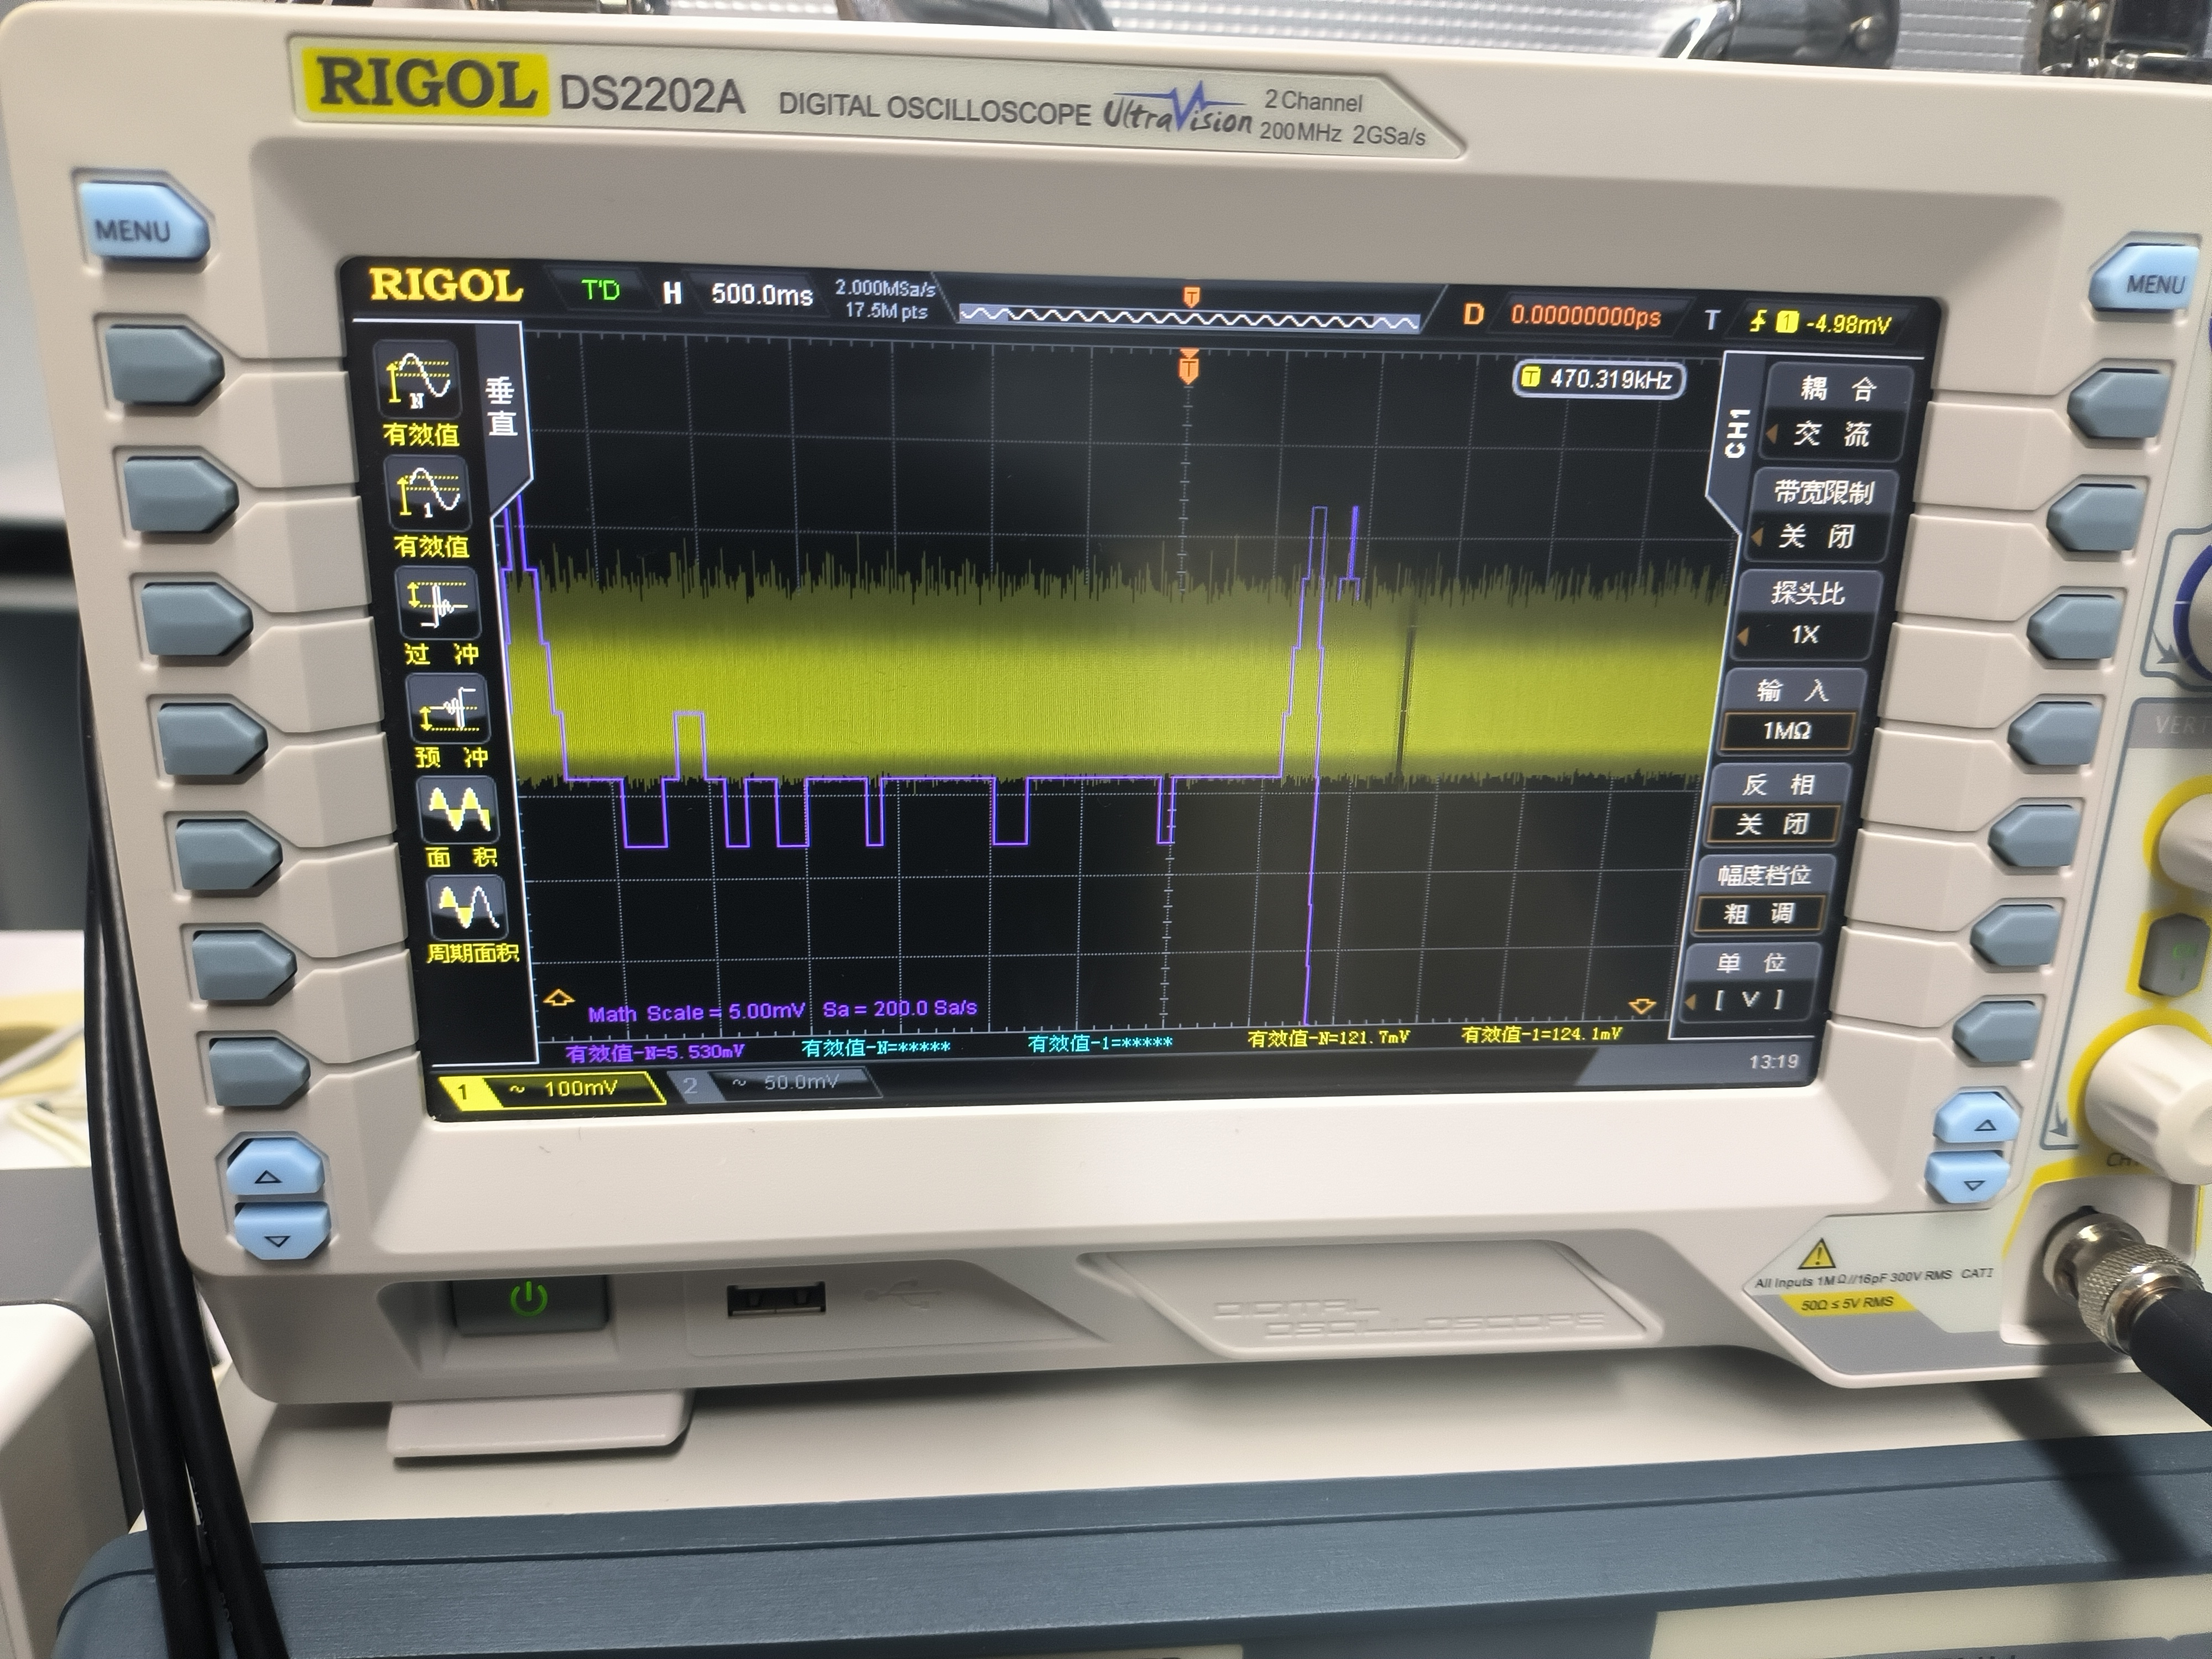
\includegraphics[width=0.4\textwidth]{D1-8-1.jpg}
	% 	\caption{噪声发生器的噪声信号测量}
	% 	\label{fig:D1-8-1}
	% \end{figure}

	\vspace{0.05\textwidth} % 两行之间的垂直间距


	\begin{table}[htbp]
		\centering
		\begin{tblr}{
		  cells = {c},
		  cell{2}{1} = {r=6}{},
		  cell{8}{1} = {r=7}{},
		  vline{1-2,4,7} = {-}{},
		  vline{4,7} = {3-7,9-14}{},
		  hline{1-2,8,15} = {-}{},
		}
		仪器    & 输入信号信噪比    & dB     & 0            & -30          & -80      \\
		示波器   & 正弦波$V_{in}$幅值 & mVrms  & 119.2        & 3.8          & -        \\
			  & 噪声信号大小     & mVrms  & 120.7        & 120.7        & 120.7    \\
			  & SNRi       & dB     & -0.11 & -30.04 & -80 \\
			  & 滤波器带宽      & Hz     & 1000         & 1000         & 1000     \\
			  & 滤波后信号有效值   & mVrms  & 135          & 4.8          & -        \\
			  & SNRo,os   & dB     & 0.97  & -28.01 & - \\
		锁相放大器 & 量程灵敏度      & mV     & 200          & 20           & 20       \\
			  & 时间常数       & ms     & 10           & 300          & 300      \\
			  & 陡降         & dB/oct & 24           & 24           & 24       \\
			  & LPF带宽      & Hz     &              &              &          \\
			  & 信号有效值R     & mVrms  & 120.1        & 3.77         & 12.1     \\
			  & 噪声有效值N     & mVrms  & 0.02         & 0.028        & 0.106    \\
			  & SNRo,lo    & dB     & 75.57  & 42.58  & 41.15  
		\end{tblr}
		\caption{强噪声背景下的弱信号检测数据}
		\label{tbl:D1-8-1}
	\end{table}



% \subsection{实验数据记录}

	% 见\cref{fig:data}

	% \begin{figure}[htbp]
	% 	\centering
	% 	\subfloat[原始数据1]
	% 	{\includegraphics[width=0.35\textwidth]{OriginalData1.jpg}\label{fig:data1}}
	% 	\quad
	% 	\subfloat[原始数据2]
	% 	{\includegraphics[width=0.35\textwidth]{OriginalData2.jpg}\label{fig:data2}}
	% 	\quad


	% 	\caption{原始数据}
	% 	\label{fig:data}
	% \end{figure}



%\subsection{原始数据记录}


\clearpage
\subsection{实验过程中遇到的问题记录}

\begin{enumerate}
	\item 由于对锁相放大器的原理理解不够透彻,导致实验进度被拖慢。
	\item 由于实验时使用的是双通道锁相放大器,而实际只用到了一条通道,需要注意设置参数时选择至实际使用的通道。
	
\end{enumerate}
	

\clearpage
\begin{table}
	\renewcommand\arraystretch{1.7}
	\begin{tabularx}{\textwidth}{|X|X|X|X|}
	\hline
	专业:& 物理学 &年级:& 2022级\\
	\hline
	姓名: & 戴鹏辉 & 学号:& 22344016\\
	\hline
    日期:& 2024/09/28 & 评分: &\\
	\hline
	\end{tabularx}
\end{table}

\section{D1 \quad 锁相放大器与弱信号测量 \quad\heiti 分析与讨论}

\subsection{实验数据分析}


	\subsubsection*{实验1.1 \quad 用示波器观察内部信号输出(与参考信号同频同相)}
		
		【问题 1】 示波器是否显示出正弦波?其测量的信号参数值是否与锁相放大器的信号设置值一致?

		由\cref{fig:D1-1-1}可知,示波器显示的是正弦波,测量的峰峰值为 $V_{pp} = 240.0 \mathrm{mV}$,即测量的有效值为
		\[
			V_{rms} = \frac{V_{pp}}{2 \sqrt{2}} = \frac{240.0 \mathrm{mV}}{2 \sqrt{2}} \approx 84.85 \mathrm{mV}
		\]

		与锁相放大器的设置值$V_{set} = 80 \mathrm{mV}$相比,可认为一致。

		同时,测量的频率$f = 1.000 \mathrm{kHz}$,与设定值一致。




	\subsubsection*{实验1.2 \quad 测量信号 $R$、$\theta$、$X$以及$Y$值,并验证它们之间的关系}

		【问题 2】 请比较示波器的读数和锁相放大器的$R$值,以理解$R$值的确切含义。

		由\cref{fig:D1-1-1}可知,锁相放大器测量的$R = 81.42 \mathrm{mV}$,与示波器测量的有效值相近,说明锁相放大器测量的$R$值为信号的有效值。


		\vspace{0.05\textwidth} % 两行之间的垂直间距


		【问题 3】 测量数据反映出$R$、$X$、$Y$及$\theta$的之间是什么关系?是否与式(D1- 22)、式(D1- 25)和(D1- 26)符合?

		由\cref{tbl:D1-2-1}的数据,有如下计算:
		\[
			R \cos\theta = 81.43 \mathrm{mV} \cdot \cos(177.33°) = -81.342 \mathrm{mV} \approx X 
		\]
		\[
			R \sin\theta = 81.43 \mathrm{mV} \cdot \sin(177.33°) = 3.793 \mathrm{mV} \approx Y 
		\]
		\[
			\sqrt{X^2 + Y^2} = \sqrt{(-81.34 \mathrm{mV})^2 + (3.79 \mathrm{mV})^2} = 81.428 \mathrm{mV} \approx R
		\]

		上式计算说明,$R$、$X$、$Y$及$\theta$的之间的关系与式(D1- 22)、式(D1- 25)和(D1- 26)符合。


		\vspace{0.05\textwidth} % 两行之间的垂直间距


		【问题 4】 你使用的 OE1022 是双锁相放大器吗?为什么?

		是双锁相放大器。因为由\cref{tbl:D1-2-1}可知,该锁相放大器可同时测量完整的输入信号信息(即信号的有效值$R$、相位角$\theta$和频率)。



	\subsubsection*{实验1.3 \quad 相敏检波器工作原理——乘法器}

		【问题 5】 示波器上看到什么波形?$X$、$Y$是正弦波吗?其相位差为多少度?$X$、$Y$的平均值为零吗?平均值是否会随滤波器参数而改变?参照式(D1-19)和式(D1-23)讨论;$R$值波形是否呈现全波整流的正弦信号,其频率为多少?与$X$或$Y$的频率存在什么关系?请对比式(D1- 28)讨论此波形。

		由\cref{fig:D1-3-3}可知,$X$、$Y$的波形并不是纯正的正弦波,而是正弦波加上了一个直流偏置,且两者之间相位相差 90°。由式(D1-19)可知,$\cos\theta$项即是直流项,$\cos(2\omega_m t + \theta)$项即是正弦波项。

		由\cref{tbl:D1-3-1}可知,增大时间常数(即改变了滤波器参数),平均值有一定变化。因为由于高频分量的存在,波形的平均值不为零。滤波器的参数(如带宽)会影响滤波效果,带宽越窄,滤波器对高频分量的抑制效果越好,输出波形的平均值越接近纯粹的直流分量。



		式(D1-19)和式(D1-23)为
		\begin{align*}
			u_{px}(t) &= \frac{1}{2} A_I s(t) \{ [ \cos((\omega_m - \omega_r)t + \theta) - \cos((\omega_m + \omega_r)t + \theta) + n(t)\sin(\omega_r t) ]\} \\
			&\approx \frac{1}{2} A_I s(t)\{ \cos\theta - \cos(2\omega_m t + \theta) + n(t)\sin(\omega_m)t\} \\
			u_{py}(t) &= \frac{1}{2} A_I s(t) [ \sin((\omega_m - \omega_r)t + \theta) + \sin((\omega_m + \omega_r)t + \theta) ]
		\end{align*}


		由\cref{fig:D1-3-1}可知,输出的双倍频正弦波类似于全波整流信号的形态,因为该信号的频率是输入信号的 2 倍。与输入信号相比,它的频率加倍。这是因为在乘法器中,输入信号与参考信号相乘会产生二次谐波成分,即频率翻倍的分量。且R与X、Y波形的频率相同。

		式(D1- 28)为
		\begin{align*}
			R(t) &= s(t) \sin(\omega_m t + \theta) \\
			&= (\sin(\omega_m t + \theta))^2 \\
			&= \frac{1 - \cos(2\omega_m t + 2\theta)}{2}
		\end{align*}





		
	\subsubsection*{实验1.4 \quad 相敏检波器工作原理——乘法器+低通滤波器}

		【问题 6】 当调大时间常数后,输出$R$是否越来越稳定?直流分量(信号平均值)是否有改变?

		调大时间常数后,锁相放大器的低通滤波器带宽减小,能够更有效地抑制高频噪声和不相关的频率成分,从而让R信号中的高频成分被滤除。所以时间常数越大,信号平均值越稳定。


		\vspace{0.05\textwidth} % 两行之间的垂直间距


		【问题 7】 观察示波器波形,并给出在某一陡降值下,时间常数为多少个信号周期时,才能观察到稳定的直流输出?提示:注意调节示波器$Y$轴量程以提高测量振幅变化的精度。并结合式(D1-32)讨论。

		式(D1-32)为
		\[
			R(t) = \frac{s(t)}{[1 + (\Delta\omega R C)^2]^{\frac{n}{2}}}
		\]

		由式(D1-32)可由以下讨论。

		\begin{enumerate}
			\item 滤波器对输入信号的影响体现在分母部分。当信号频率与参考频率不一致时,存在频率偏差 \( \Delta\omega \),信号 \( R(t) \) 随着频率偏差增大而衰减。

			\[\text{当 } \Delta\omega = 0 \text{ 时,} R(t) = s(t) \text{,即信号未受衰减。}\]

			\[\text{当 } \Delta\omega \neq 0 \text{ 时,滤波器开始衰减信号。频率偏差越大,衰减越严重。}\]

			时间常数 \( \tau = RC \) 越大,带宽越窄,滤波器可以更好地滤除偏离频率的成分,增强信号稳定性。

			\item **滤波器阶数 \( n \) 的影响**:

			滤波器的阶数 \( n \) 决定了信号幅度随频率偏差 \( \Delta\omega \) 的衰减速度。

			\[\text{低阶滤波器:} n = 1 \text{(6 dB/oct),信号衰减较慢,允许更大的频率偏差。}\]

			\[\text{高阶滤波器:} n = 4 \text{(24 dB/oct),信号衰减快,频率稍有偏差时信号就会显著衰减。}\]

			高阶滤波器有助于滤除噪声,使信号更稳定。

			\item **时间常数与信号稳定性的关系**:

			随着时间常数 \( \tau = RC \) 的增大,公式中的项 \( (\Delta\omega R C)^2 \) 也会增大,滤波器能够更有效地抑制偏离中心频率的信号成分,使 \( R(t) \) 越来越稳定。

			\item **信噪比的影响**:

			通过调节滤波器带宽(即时间常数 \( RC \)),可以提高信号的信噪比。带宽越窄,滤波器允许通过的频率范围越小,从而滤除更多的噪声。时间常数越大,带宽越窄,信噪比提高,信号更加稳定。

		\end{enumerate}

		


		\vspace{0.05\textwidth} % 两行之间的垂直间距



		【问题 8】为何在 1 阶(6dB/oct)时还没怎么起滤波效果,而到 4 阶(24dB/oct)时,则可看见明显的效果?

		观察\cref{fig:D1-4-1-1}、\cref{fig:D1-4-1-2}、\cref{fig:D1-4-1-3}、\cref{fig:D1-4-1-4},可以发现,陡降设置的越大,输出波形的幅值越小,滤波效果越明显。

		陡降表示信号在截止频率处的衰减速度,滤波器的阶数越高,陡降越陡,能更有效地去除高频噪声。所以,陡降越陡,滤波器在其截止频率附近的频率选择性就越好,即滤波效果越明显。





	\subsubsection*{实验1.8 \quad 强噪声背景下的弱信号检测}

		【问题 12】如何获得幅值为 0.1mVrms 的正弦波输入信号?

		由于信号发生器最低只能设置 0.7mVrms 的正弦波输入信号,所以需要考虑其他方式获得幅值为 0.1mVrms 的正弦波输入信号。

		可以考虑使用噪声发生器的信号端接口的 -80dB 的衰减开关,通过一个较大的信号经过衰减之后得到所需的信号。
		\[
			- 80 \mathrm{dB} = 20 \log \frac{V_{out}}{V_{in}} = 20 \log \frac{0.1 \mathrm{mVrms}}{V_{in}}
		\]
		\[
			\Rightarrow V_{in} = 10000 \times 0.1 \mathrm{mVrms} = 1 \mathrm{Vrms}
		\]

		即,可以使用信号发生器产生一个 1 Vrms 的正弦波信号,再经过噪声发生器的信号端接口的 -80dB 的衰减,即可得到幅值为 0.1mVrms 的正弦波输入信号。


		\vspace{0.05\textwidth} % 两行之间的垂直间距


		【问题 13】对低信噪比信号或非周期噪声测量,能否用示波器的“auto”键?若通过手动调节,示波器屏宽(时间轴范围)应为多少个信号周期为宜?

		示波器的“auto”模式会首先检测输入信号的特征,包括频率、幅度和波形类型,根据信号的周期性,示波器会自动选择合适的时间轴范围,以确保信号在屏幕上完整显示;而非周期信号本身缺乏稳定的重复模式,因此很难通过自动设置来捕捉到完整的信号特征。

		手动调节时,建议设置为 2-5 个周期,因为过少的周期可能导致信号不够稳定,无法有效判断信号特征,而过多的周期则可能导致信号在屏幕上变得拥挤,影响观察效果。


		\vspace{0.05\textwidth} % 两行之间的垂直间距


		【问题 14】在用示波器观察、测量信号有效值时,请注意屏幕时间轴范围应达到待观测信号完整周期的整数倍;为什么?

		因为信号有效值的计算基于信号的平方在时间上的平均,即
		\[
			u_{rms} = \frac{\int_0^{t} (u(\tau))^2 \mathrm{d\tau}}{t} \approx \frac{\int_0^{nT} (u(\tau))^2 \mathrm{d\tau}}{nT} = \frac{n\int_0^{T} (u(\tau))^2 \mathrm{d\tau}}{nT} = \frac{\int_0^{T} (u(\tau))^2 \mathrm{d\tau}}{T}
		\]

		其中,“$\approx$”仅在“积分时间$t$远大于周期$T$”,或“积分时间$t$是周期$T$的整数倍”时才成立。

		所以,屏幕时间轴范围应达到待观测信号完整周期的整数倍。


		\vspace{0.05\textwidth} % 两行之间的垂直间距


		【问题 15】用锁相放大器测量 $R$ 值时,读数应保留几位有效数字?调节锁相放大器的什么参数设置可以得到?调节锁相放大器的什么参数可以获得稳定的读数。

		读数应在取得2-3位稳定示数后,保留2-3位有效数字。通过设置合适的Sensitivity,可以使得有效数字位数显示的尽可能多且保证一定的测量精度。

		通过设置合适的时间常数和陡降,可以获得稳定的读数。




\subsection{实验报告思考题}


% 思考题1
\begin{question}
	描述用教学实验箱配制不同信噪比信号的原理;实验箱生成的噪声是否为白噪声?
\end{question}

	教学实验箱可以产生有效值恒定的噪声(若设备良好则为100mVrms);同时,实验箱上配有两个10dB的衰减开关,可以通过不同的开关组合,得到10mVrms、1mVrms的噪声;对于信号发生器,其自生可以产生0.7mVrms-5Vrms的信号,通过实验箱上80dB的衰减开关,最低可以得到70nVrms的信号。通过信号与噪声的不同混合,可以得到信噪比不同的待测信号。

	实验箱生成的是白噪声。因为其在频域下的不同频率的功率谱密度基本相同,没有特殊频率的倾向。






% 思考题2
\begin{question}
	随着信噪比的改变,信号 $R$ 和相位差$\theta$的测量值会有什么影响?
\end{question}

	信噪比的计算公式为
	\[
		\mathrm{SNR} = 10\log\frac{V_{S,RMS}^2}{R^2 - V_{S,RMS}^2}
	\]
	\[
		\Rightarrow V_{S,RMS}^2 = \frac{1}{10^{-\frac{\mathrm{SNR}}{10}} + 1} R^2
	\]

	则:
	\begin{enumerate}
		\item 当信噪比较高时,测量得到的有效值$R$基本等于信号值$V_{S,RMS}$。
		\item 信噪比较低时,噪声对有效值的贡献显著,测得的值会高于实际信号有效值,噪声越大偏离越严重。
	\end{enumerate}

	相位差的测量也会受到噪声的影响,尤其当信噪比降低时,噪声对相位的干扰会显著增加。信号和噪声的相位分别为$\theta_{S}$和$\theta_{N}$,测得的相位差$\theta_{M}$可以表示为信号和噪声的组合结果:
	\[
		\tan \theta_{M} = \frac{V_{S,RMS}\sin\theta_{S} + V_{N,RMS}\sin\theta_{N}}{V_{S,RMS}\cos\theta_{S} + V_{N,RMS}\cos\theta_{N}}
	\]

	同样的,当信噪比高时,噪声项的影响较小;当信噪比低时,噪声项会对测量结果产生较大干扰,导致相位测量值不稳定,甚至会发生显著偏差或跳变。相位差测量的不确定性和噪声水平成正比。


% 思考题3
\begin{question}
	所有的噪声都可以用锁相放大器消除吗?锁相放大器的理论检测极限是多少?受什么限制?
\end{question}

	锁相放大器通过同步检测原理,可以有效地抑制与信号频率无关的噪声;与之相对的,如果噪声与待测信号的频率接近或相同,锁相放大器可能难以区分并抑制这些噪声。此外,由于锁相放大器依赖信号的相位,若信号的相位受到随机扰动(相位噪声)的影响,锁相放大器的输出也会受到干扰。

	锁相放大器的理论检测极限通常由其最小可测信号决定,即能够在给定信噪比下从噪声中分离出来的最小信号强度。这个极限受以下几个主要因素的限制:
	\begin{enumerate}
		\item 输入噪声:锁相放大器的输入放大器本身会引入一定的噪声,通常称为“输入噪声电平”。该噪声电平会限制能够检测到的最小信号。如果输入噪声电平很高,低于此噪声电平的信号将难以检测到。
		\item 带宽:滤波器带宽越窄,噪声抑制能力越强,但这也可能导致信号响应变慢。理论上,带宽越窄,锁相放大器越能从噪声中分离出微弱的信号。然而,带宽太窄时会导致响应时间过长,因此存在折中。
		
		锁相放大器的最小可测信号与带宽 $B$ 的关系通常为:
		\[
			S_{min} \propto \frac{N}{\sqrt{B}}
		\]
		其中$S_{min}$是最小可测信号,$N$是输入噪声电平,$B$是滤波带宽。

		\item 参考信号的稳定性:锁相放大器的工作依赖于参考信号的频率和相位,如果参考信号不稳定(如存在频率漂移或相位噪声),会影响锁相放大器的检测能力。
		\item 相位噪声:如果待测信号或参考信号存在相位噪声,锁相放大器的相位测量会不稳定,从而影响信号检测的精度。
	\end{enumerate}




% 思考题4
\begin{question}
	请比较锁相放大器与示波器(经过带通滤波后)测量不同信噪比信号的结果,分析两种测量仪器(方法)的优势与劣势。选择锁相放大器窄带宽的 LPF 可以降低式(D1- 34)中的$n_{\omega_r}$,从而提高测量值的信噪比吗?信噪比的提高与 LPF 带宽有何关系?参考式(D1-10)讨论。
\end{question}

	锁相放大器和示波器(经过带通滤波后)在测量不同信噪比信号时具有不同的优势与劣势。

	\begin{enumerate}

		\item \textbf{锁相放大器的优势与劣势}

		\textbf{优势}:
		\begin{itemize}
			\item 锁相放大器通过相干检测,可以有效提取特定频率的信号,尤其适用于在低信噪比下提取微弱信号。
			\item 锁相放大器的窄带低通滤波器(LPF)可以极大减少带外噪声,从而提高信号的信噪比(SNR)。
		\end{itemize}

		\textbf{劣势}:
		\begin{itemize}
			\item 锁相放大器的测量频率范围受限于参考信号频率,因此不适用于宽频范围内的信号测量。
			\item 在非相干噪声较强时,锁相放大器的效果可能不如预期。
		\end{itemize}

		\item \textbf{示波器(带通滤波后)的优势与劣势}

		\textbf{优势}:
		\begin{itemize}
			\item 示波器具有宽频响应能力,能够实时显示并分析多频段的信号。
			\item 经过带通滤波后,示波器可以减少带外噪声,从而对特定频率信号进行较为准确的测量。
		\end{itemize}

		\textbf{劣势}:
		\begin{itemize}
			\item 即使经过带通滤波,示波器仍可能受到带内噪声的影响,特别是在信号较弱且噪声较强的情况下,信噪比不易得到显著提升。
			\item 示波器本身没有相干检测的能力,不能有效区分相干噪声和信号。
		\end{itemize}

		\item \textbf{LPF 带宽与信噪比的关系}

		锁相放大器使用窄带低通滤波器(LPF)确实可以降低公式(D1-34)中的噪声成分 $n_{\omega_r}$,从而提高测量值的信噪比。

		在锁相放大器中,输出信号的噪声功率 $n_{\omega_r}$ 与低通滤波器的带宽 $B$ 成正比,因此信噪比 $\text{SNR}$ 可以通过减小带宽 $B$ 来提高。具体来说,信噪比与带宽的关系可以表示为:

		\[
		\text{SNR} \propto \frac{1}{B}
		\]

		因此,锁相放大器选择窄带宽的低通滤波器可以有效提高信噪比。但带宽过窄也会导致响应时间变长,可能影响测量的实时性。

		\item \textbf{结论}

		锁相放大器适用于低信噪比、特定频率的信号提取,而示波器在宽频率信号分析中具有优势。锁相放大器通过减小低通滤波器的带宽可以有效提高信噪比,但也需要在带宽和响应时间之间找到平衡。

	\end{enumerate}



\end{document}
